\documentclass[12pt]{article}
\usepackage[utf8]{inputenc}
\usepackage{parskip}
\usepackage[spanish]{babel}
\usepackage{amsmath, amssymb}
\usepackage{graphicx}
\usepackage{makecell}
\usepackage{geometry}
\usepackage{caption}
\usepackage{float}
\usepackage[hidelinks]{hyperref}
\usepackage{enumitem}

% --------------------- Comandos para pie de página ---------------------
\usepackage[backend=biber, bibstyle=apa, citestyle=numeric]{biblatex}
\usepackage{csquotes}
%\addbibresource{referencias.bib}
%\usepackage{hyperref}
%\usepackage{url}

%\makeatletter
%\g@addto@macro{\UrlBreaks}{\UrlOrds}
%\makeatother

%\renewcommand{\footnoterule}{%
%  \kern -3pt                         % Espacio vertical sobre la línea
%  \hrule width \textwidth height 0.4pt % Ancho total de la página y grosor
%  \kern 2.6pt                        % Espacio vertical debajo de la línea
%}
% -----------------------------------------------------------------------
\addbibresource{referencias.bib}
\geometry{letterpaper, margin=2.5cm}
\setlength{\parskip}{1em}

\begin{document}
\begin{titlepage}
\begin{center}
    % Logos
    \begin{minipage}{0.3\textwidth}
        
\includegraphics[width=0.8\linewidth]{imagenes/UNAM_Logo.png}
    \end{minipage}\hfill
    \begin{minipage}{0.4\textwidth}
        \begin{center}
            \textbf{\Large Universidad Nacional Autónoma de México}\\[0.2cm]
            \textbf{Facultad de Ciencias}\\[0.2cm]
        \textbf{Bases de Datos}
        \end{center}
    \end{minipage}\hfill
    \begin{minipage}{0.3\textwidth}
        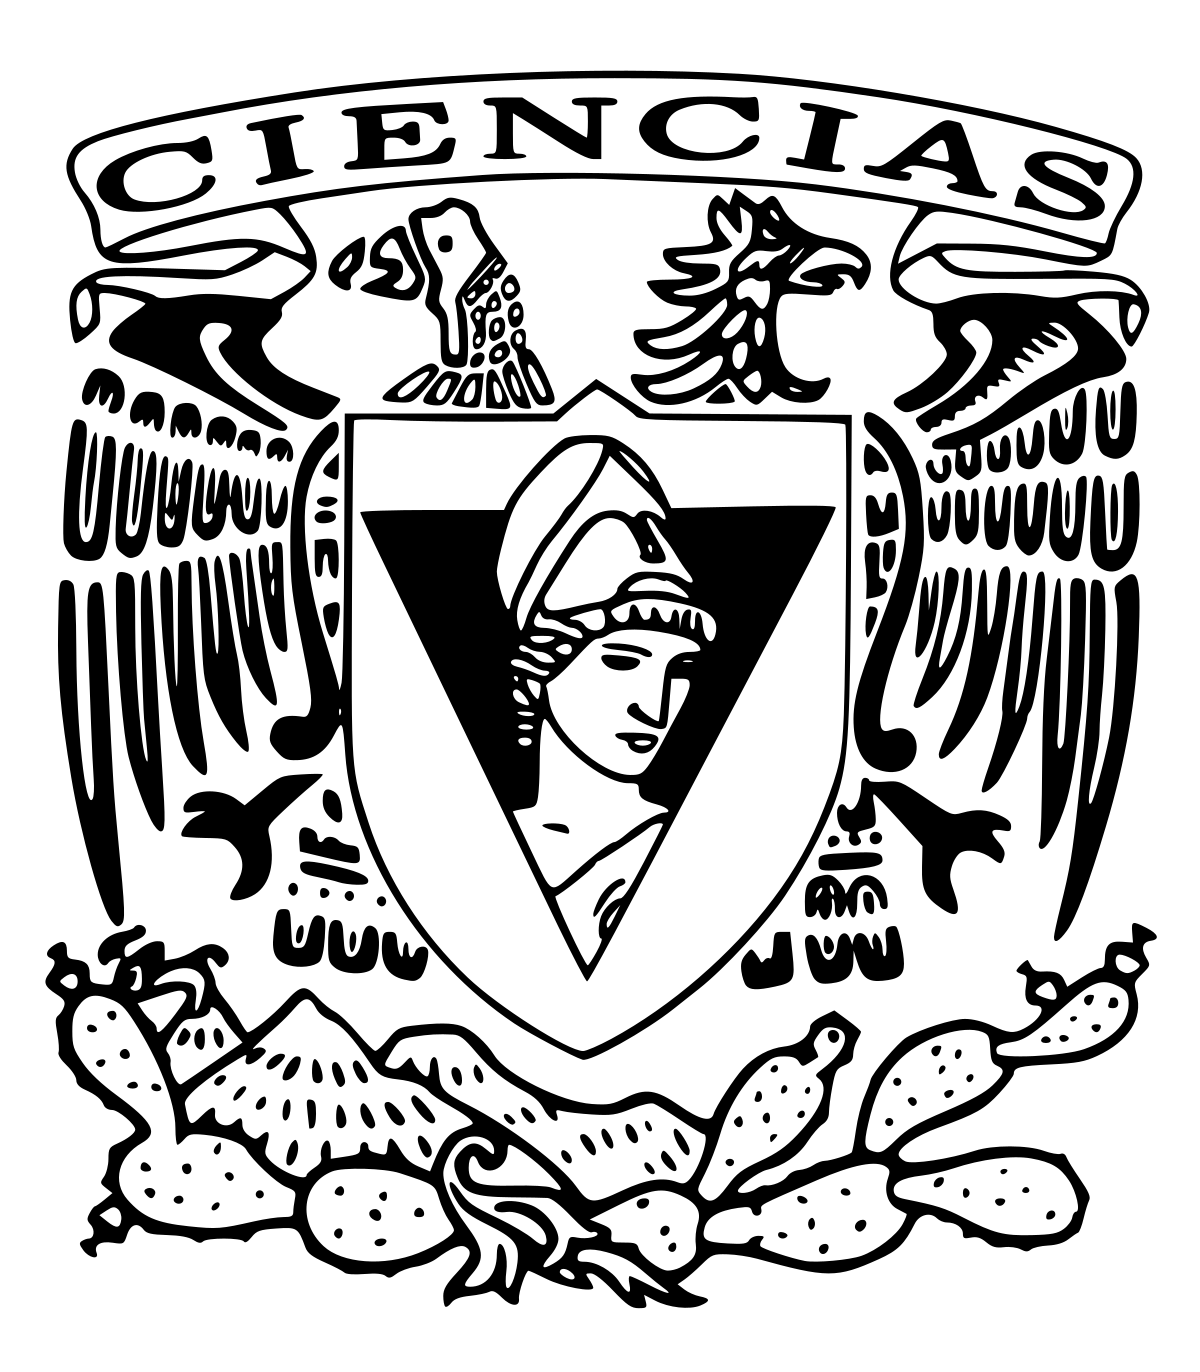
\includegraphics[width=0.8\linewidth]{imagenes/Logo_FC.png}
    \end{minipage}
    \vspace{3cm}
    \textbf{\large Tarea 4}\\
    Licenciatura en Ciencias de la Computación\\
    Profesor: Gerardo Avilés Rosas \\
    \vspace{2cm}
    \textbf{Integrantes: }\\
    Cisneros Tenorio Diego Alexander\\
    Nuñez Ruiz José Manuel \\
    Olmos Ortiz Andrea Lucia\\
    Reynoso Ascencio Alexa \\
    Vega Navas Saúl \\
    \vspace{2cm}
    \textbf{Fecha de entrega: } 30 de Octubre del 2026
    \vfill
\end{center}
\end{titlepage}
\tableofcontents
% Preguntas

% Ejercicio 1
 \section*{1. Cardinalidad de la consulta}
\addcontentsline{toc}{section}{1. Cardinalidad de la consulta}

Considera las siguientes relaciones:

\vspace{0.5cm}

\begin{center}
\begin{minipage}{0.35\textwidth}
  \centering
  $R =$ \quad
  \begin{tabular}{|c|c|}
    \hline
    \textbf{A} & \textbf{B} \\ \hline
    1 & x \\
    2 & y \\
    2 & z \\
    3 & x \\
    9 & a \\ \hline
  \end{tabular}
\end{minipage}
\begin{minipage}{0.45\textwidth}
  \centering
  $S =$ \quad
  \begin{tabular}{|c|c|c|}
    \hline
    \textbf{B} & \textbf{C} & \textbf{D} \\ \hline
    x & 0 & 3 \\
    y & 2 & 1 \\
    y & 3 & 3 \\
    w & 3 & 0 \\
    y & 4 & 2 \\ \hline
  \end{tabular}
\end{minipage}
\end{center}

\vspace{0.5cm}

Para las siguientes expresiones de \textbf{álgebra relacional}, completa la tabla con el número de tuplas que cada una de ellas produce utilizando las relaciones \textbf{R} y \textbf{S}. Deberás indicar las \textbf{tablas resultantes} en cada caso.

\vspace{0.5cm}

\begin{center}
\begin{tabular}{|l|p{5cm}|}
  \hline
  \textbf{Expresión} & \textbf{Cardinalidad del resultado} \\ \hline
  $R \times S$ & \\ \hline
  $R \bowtie_{D > A} S$ & \\ \hline
  $R \rtimes S$ & \\ \hline
  $R \ltimes S$ & \\ \hline
  $R \bowtie_{A = D} S$ & \\ \hline
  $\rho_{C \leftarrow A}(R) \bowtie S$ & \\ \hline
  $\pi_B(R) - \pi_B(\sigma_{C \ge 3}(S))$ & \\ \hline
  $\pi_A(R) \cap \rho_{A \leftarrow D}(\pi_D(S))$ & \\ \hline
  $\pi_D(S) \bowtie R$ & \\ \hline
  $\gamma_{A; \text{count}(B) \rightarrow t}(R \bowtie S)$ & \\ \hline
\end{tabular}
\end{center}

 \subsection*{Justificacion Fila 2:}

La operación indica tomar las filas del producto cartesiano del inciso anterior que cumplan con la propiedad expresada \texttt{S,D>R.A}, de lo que se obtiene:

\begin{center}
$R \bowtie_{D > A} S =$ \quad
\begin{tabular}{|c|c|c|c|c|}
\hline
\textbf{A} & \textbf{R.B} & \textbf{S.B} & \textbf{C} & \textbf{D} \\ \hline
  1 & x & x & 0 & 3 \\
  1 & x & y & 3 & 3 \\
  1 & x & y & 4 & 2 \\
  2 & y & x & 0 & 3 \\
  2 & y & y & 3 & 3 \\
  2 & z & x & 0 & 3 \\
  2 & z & y & 3 & 3 \\ \hline
\end{tabular}
\end{center}

Por lo tanto, la cardinalidad del resultado es \textbf{6}.
 \subsection*{Justificación Fila 3}

El join externo por la izquierda conserva todas las tuplas de la relación de la izquierda ($R$), así como las combinaciones que hicieron coincidencia en el join natural con $S$. Si una tupla de $R$ no tiene coincidencia, los atributos de $S$ en el resultado se rellenan con valores nulos (NULL).

Ambas tablas comparten el atributo $B$. Primero obtenemos las coincidencias exactas (Join Natural $R \bowtie S$):
\begin{itemize}
    \item Para $B = x$: $(1, x)$ y $(3, x)$ en $R$ coinciden con $(x, 0, 3)$ en $S$. Se generan 2 tuplas.
    \item Para $B = y$: $(2, y)$ en $R$ coincide con $(y, 1, 2), (y, 3, 3)$ y $(y, 4, 2)$ en $S$. Se generan 3 tuplas.
\end{itemize}
Total de coincidencias: 5 tuplas.

A continuación, revisamos las tuplas de $R$ que no hicieron match con $S$:
\begin{itemize}
    \item $(2, z)$ en $R$ (no hay $z$ en la columna $B$ de $S$).
    \item $(9, a)$ en $R$ (no hay $a$ en la columna $B$ de $S$).
\end{itemize}
Estas 2 tuplas se conservan en el resultado y se completan con NULL.

Por lo tanto, la cardinalidad del resultado es $5 + 2 = \mathbf{7}$ \textbf{tuplas}.

\begin{center}
$(R =\bowtie S) =$ \quad
\begin{tabular}{|c|c|c|c|}
\hline
\textbf{A} & \textbf{B} & \textbf{C} & \textbf{D} \\ \hline
1 & x & 0 & 3 \\
3 & x & 0 & 3 \\
2 & y & 1 & 2 \\
2 & y & 3 & 3 \\
2 & y & 4 & 2 \\
2 & z & \text{NULL} & \text{NULL} \\
9 & a & \text{NULL} & \text{NULL} \\ \hline
\end{tabular}
\end{center}

 \subsection*{Justificación Fila 4}

El join por la derecha conserva todas las tuplas de la relación de la derecha ($S$), además de las coincidencias del join natural. Las tuplas de $S$ que no tienen coincidencia con $R$ se conservan y se rellenan con nulos (NULL) en los atributos correspondientes a $R$.

Las coincidencias naturales ya las calculamos en el paso anterior y sabemos que nos dan 5 tuplas. Revisamos las tuplas de $S$ que no hicieron match con $R$:
\begin{itemize}
    \item $(w, 3, 0)$ en $S$ (no hay valor $w$ en la columna $B$ de $R$).
\end{itemize}
Esta única tupla se conserva y se rellena con NULL para la columna $A$ de $R$.

Por lo tanto, la cardinalidad del resultado es $5 + 1 = \mathbf{6}$ \textbf{tuplas}.

\begin{center}
$(R \bowtie= S) =$ \quad
\begin{tabular}{|c|c|c|c|}
\hline
\textbf{A} & \textbf{B} & \textbf{C} & \textbf{D} \\ \hline
1 & x & 0 & 3 \\
3 & x & 0 & 3 \\
2 & y & 1 & 2 \\
2 & y & 3 & 3 \\
2 & y & 4 & 2 \\
\text{NULL} & w & 3 & 0 \\ \hline
\end{tabular}
\end{center}

 \subsection*{Justificacion Fila 5:}
  \[R \bowtie_{A = D} S\]


  
\begin{center}
\begin{tabular}{|c|c|c|c|c|}
  \hline
  \textbf{A} & \textbf{R.B} & \textbf{S.B} & \textbf{C} & \textbf{D} \\ \hline
  1 & x & y & 2 & 1 \\ \hline
  2 & y & y & 4 & 2 \\ \hline
  2 & z & y & 4 & 2 \\ \hline
  3 & x & x & 0 & 3 \\ \hline
  3 & x & y & 3 & 3 \\ \hline
  9 & a & NULL & NULL & NULL \\ \hline
\end{tabular}
\end{center}

Hay\textbf{ 5 }tuplas en $ R \times S$ que cumplen con $A = D$.\\
 \subsection*{Justificacion Fila 6:}

Primero se renombra la fila A de la tabla R, por el nombre C.

\begin{center}
$\rho_{C \leftarrow A}(R) = R'=$ \quad
\begin{tabular}{|c|c|}
  \hline
  \textbf{C} & \textbf{B} \\ \hline
  1 & x \\
  2 & y \\
  2 & z \\
  3 & x \\
  9 & a \\ \hline
\end{tabular}
\end{center}

Posteriormente se aplica Join Natural sobre la tabla anterior y la tabla S. Dado que las tablas comparten las columnas C y B, entonces con el join natural buscamos las tuplas en donde los valores de estas columnas coinciden. Notemos que solo coinciden para $C = 2$ y $B = y$). Así, tenemos la siguiente tabla.
\begin{center}
$R' \bowtie S =$ \quad
\begin{tabular}{|c|c|c|}
  \hline
 
  \textbf{C} & \textbf{B} & \textbf{D} \\ \hline
  2 & y & 1 \\ \hline
\end{tabular}
\end{center}

 \subsection*{Justificacion Fila 7:}

La operación indica tomar la columna \texttt{R.B}, y luego restarle las celdas de la columna \texttt{S.B} tales que su respectivo registro \texttt{S.C} sea mayor o igual a 3.
\begin{center}
\begin{tabular}{c c c c c c c c}
    $\pi_B(R) =$
&
\begin{tabular}{|c|}
\hline
\textbf{B} \\ \hline
  x
  \\
  y
  \\
  z
  \\
  x
  \\
  a 
  \\ \hline
\end{tabular}
& &     $\pi_B(\sigma_{C \ge 3}(S)) =$ &
\begin{tabular}{|c|}
\hline
\textbf{B} \\ \hline
  y
  \\
  w
  \\
  y
  \\ \hline
\end{tabular}
& &     $\pi_B(R)-\pi_B(\sigma_{C \ge 3}(S)) =$ &
\begin{tabular}{|c|}
\hline
\textbf{B} \\ \hline
  x
  \\
  z
  \\
  a
  \\ \hline
\end{tabular}
\end{tabular}
\end{center}

Por lo tanto, la cardinalidad del resultado es \textbf{3}.
 \subsection*{Justificacion Fila 8:}

Primero se proyecta la columna $A$ de $R$. Eliminamos los renglones duplicados, en este caso eliminamos un $2$ ya que aparece dos veces.

\begin{center}
$\pi_{A}(R) =$ \quad
\begin{tabular}{|c|}
\hline
\textbf{A} \\ \hline
  1 \\
  2 \\
  3 \\
  9 \\ \hline
\end{tabular}
\end{center}

Después se proyecta la columna $D$ de $S$. De igual forma, eliminamos un $3$ ya que aparece dos veces.

\begin{center}
$\pi_{D}(S) =$ \quad
\begin{tabular}{|c|}
\hline
\textbf{D} \\ \hline
  3 \\
  1 \\
  0 \\
  2 \\ \hline
\end{tabular}
\end{center}

Se renombra la columna $D$ por $A$ para poder aplicar la intersección, ya que se requiere que los atributos tengan el mismo nombre.

\begin{center}
$\rho_{A \leftarrow D}(\pi_{D}(S)) =$ \quad
\begin{tabular}{|c|}
\hline
\textbf{A} \\ \hline
  3 \\
  1 \\
  0 \\
  2 \\ \hline
\end{tabular}
\end{center}

Se aplica la intersección, que conserva únicamente los valores que aparecen en ambas tablas. Por lo que como $9$ solo está en la primera y $0$ solo en la segunda, estos valores los eliminamos.

\begin{center}
$\pi_{A}(R) \cap \rho_{A \leftarrow D}(\pi_{D}(S)) =$ \quad
\begin{tabular}{|c|}
\hline
\textbf{A} \\ \hline
  1 \\
  2 \\
  3 \\ \hline
\end{tabular}
\end{center}

Por lo tanto, la cardinalidad del resultado es \textbf{3}.
 \subsection*{Justificacion Fila 9:}

\[\pi_D(S) \bowtie R\]

Primero se proyecta la columna $D$ de $S$. Eliminamos los renglones duplicados, eliminamos un $3$ ya que aparece dos veces.

\begin{center}
$\pi_{D}(S) =$ \quad
\begin{tabular}{|c|}
\hline
\textbf{D} \\ \hline
  3 \\
  1 \\
  0 \\
  2 \\ \hline
\end{tabular}
\end{center}

\begin{center}
\begin{minipage}{0.35\textwidth}
  \centering
  $R =$ \quad
  \begin{tabular}{|c|c|}
    \hline
    \textbf{A} & \textbf{B} \\ \hline
    1 & x \\
    2 & y \\
    2 & z \\
    3 & x \\
    9 & a \\ \hline
  \end{tabular}
\end{minipage}
\end{center}

$\pi_{D}(S) $ no comparte atributos con $R$, así que el join natural equivale al producto cartesiano.
\[4 \times 5 = \text{\textbf{20}}\]
 \subsection*{Justificacion Fila 10}

Primero se obtiene la tabla sobre la que vamos a aplicar la agrupación. Para esto calculamos el join externo de ambas tablas, en donde conservamos todos los elementos de cada tabla y rellenamos con valores nulos.

\begin{center}
$(R =\Join= S) = T =$ \quad
\begin{tabular}{|c|c|c|c|}
  \hline
  \textbf{A} & \textbf{B} & \textbf{C} & \textbf{D} \\ \hline
  1 & x & 0 & 3 \\
  2 & y & 2 & 1 \\
  2 & y & 3 & 3 \\
  2 & y & 4 & 2 \\
  2 & z & \text{NULL} & \text{NULL} \\
  3 & x & 0 & 3 \\
  9 & a & \text{NULL} & \text{NULL} \\
  \text{NULL} & w & 3 & 0 \\ \hline
\end{tabular}
\end{center}

Posteriormente, aplicamos la agrupación respecto a la columna A, contando cuántas filas con valores no nulos respecto a B tiene cada valor de A. De este modo obtenemos una nueva tabla con las columnas de los valores de A y el número de veces que se repite (t).

\begin{center}
$\gamma_{A; \text{count}(B) \rightarrow t}T=$ \quad
\begin{tabular}{|c|c|}
  \hline
  \textbf{A} & \textbf{t} \\ \hline
  1 & 1 \\
  2 & 4 \\
  3 & 1 \\
  9 & 1 \\
  \text{NULL} & 1 \\ \hline
\end{tabular}
\end{center}


% Ejercicio 2
 \section*{2. Tienda de productos en línea}
\addcontentsline{toc}{section}{2. Tienda de productos en línea}
 \subsection*{b. Obtener una relación de los productos que pertenecen a la categoría Technology con precio mayor de \$400 y menor de \$850, pero que no hayan sido solicitados en ninguna orden.}

Primero seleccionamos los productos de la categoría \textit{Technology} cuyo precio sea mayor a 400 y menor a 850. Después obtenemos los id de los productos que sí han sido solicitados en alguna orden; restamos estos id a los de los productos seleccionados, por lo que quedan únicamente los productos que no han sido solicitados. Realizamos un join natural con la tabla \textit{products} para recuperar toda la información de los productos

Expresión:
\begin{equation}
\left( \pi_{productid}\left(\sigma_{category = \text{'Technology'} \, \wedge \, price > 400 \, \wedge \, price < 850}(products)\right) - \pi_{productid}(orders) \right) \bowtie products
\end{equation}

Resultados obtenidos:

\begin{figure}[h!]
\centering
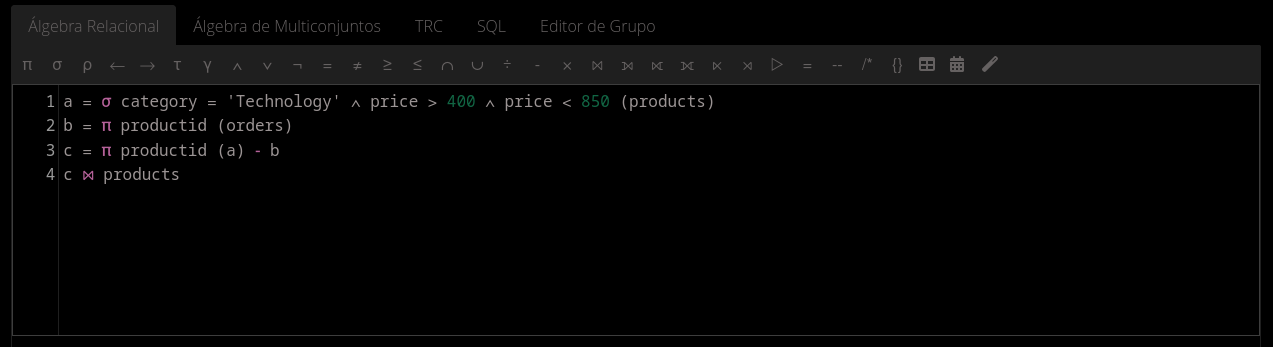
\includegraphics[width=0.8\textwidth]{imagenes/2b(1).png}
\caption{Consulta}
\end{figure}

\begin{figure}[h!]
\centering
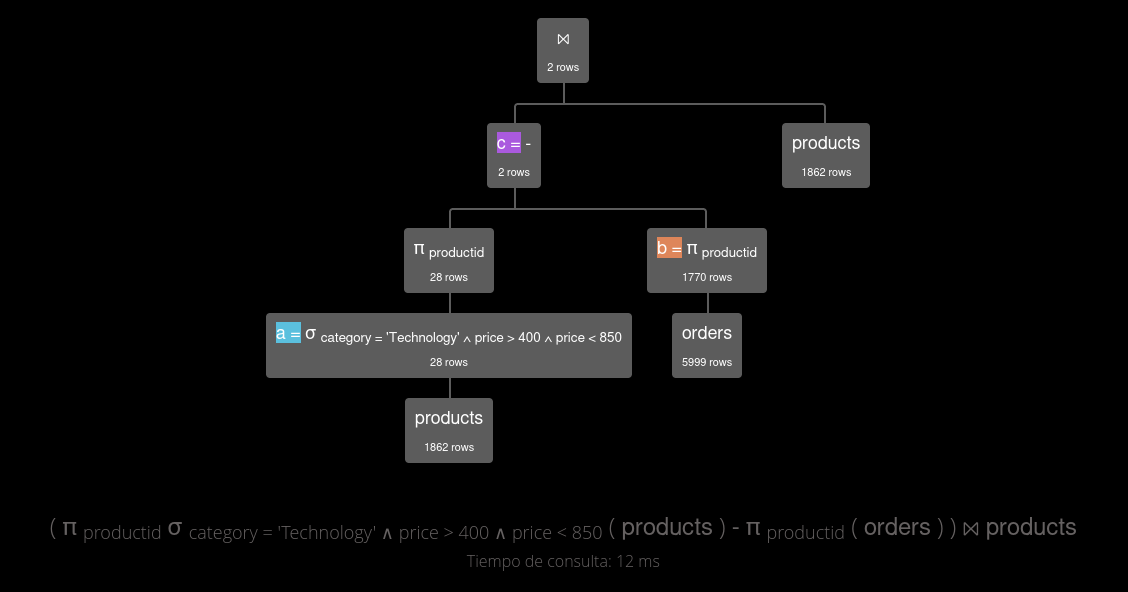
\includegraphics[width=0.8\textwidth]{imagenes/2b(2).png}
\caption{Árbol de consulta.}
\end{figure}

\begin{figure}[h!]
\centering
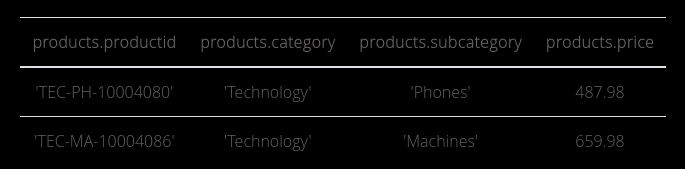
\includegraphics[width=0.6\textwidth]{imagenes/2b(3).png}
\caption{Resultado de consulta.}
\end{figure}
 \subsection*{c. Obtener el nombre de todos los clientes que vivan en la región South y hayan solicitados productos de las subcategorías Bookcases o Chairs o Appliances o Copiers. El pedido debió de solicitarse el primer o tercer trimestre de 2015 y el modo de envío debe ser Standard Class.}

Renombramos las tablas \textit{customer}, \textit{orders} y \textit{products} como $c$, $o$ y $p$ respectivamente. Después realizamos un join entre $c$ y $o$ con el id del cliente, y al resultado le aplicamos otro join con $p$ con el id del producto, así cada fila tendrá la información del cliente, de la orden y del producto. \\ \\
Luego, proyectamos únicamente el nombre del cliente para obtener la lista de clientes que cumplen con todas las condiciones.

Expresión:
\[
\begin{aligned}
&\pi_{c.customername}\Bigg(
  \sigma_{\substack{
    c.region = \text{'South'} \;\\
    \land\; o.shipmode = \text{'Standard Class'} \; \\
    \land\;\big(\, (o.shipdate \geq \text{DATE('2015-01-01')} \;\land\; o.shipdate < \text{DATE('2015-04-01')}) \\
    \lor\; (o.shipdate > \text{DATE('2015-06-30')} \;\land\; o.shipdate < \text{DATE('2015-10-01')}) \,\big) \; \\
    \land\; \big(\, p.category = \text{'Bookcases'} \lor p.category = \text{'Chairs'} \\
                \lor\; p.category = \text{'Appliances'} \lor p.category = \text{'Copiers'} \,\big)
  }} \\
&\qquad\Big(
  \big( \rho_{c}(customer) \bowtie_{c.customerid = o.customerid} \rho_{o}(orders) \big)
  \bowtie_{o.productid = p.productid} \rho_{p}(products)
\Big)\Bigg)
\end{aligned}
\]
Resultados obtenidos:

\begin{figure}[h!]
\centering
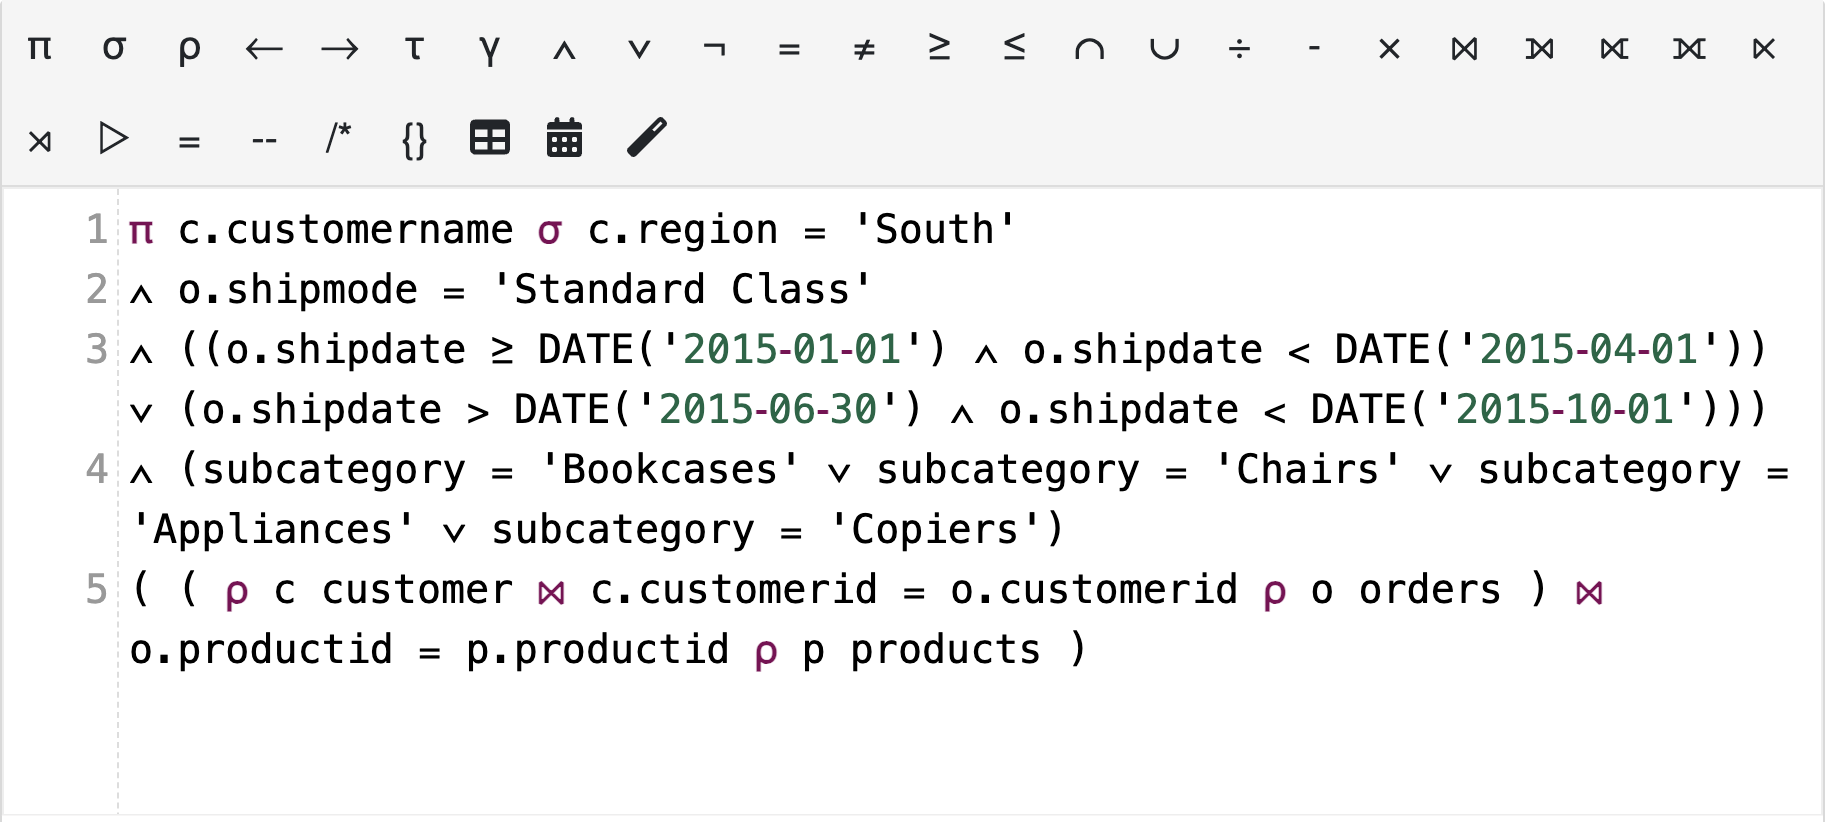
\includegraphics[width=0.8\textwidth]{imagenes/2c(1).png}
\caption{Consulta}
\end{figure}

\begin{figure}[h!]
\centering
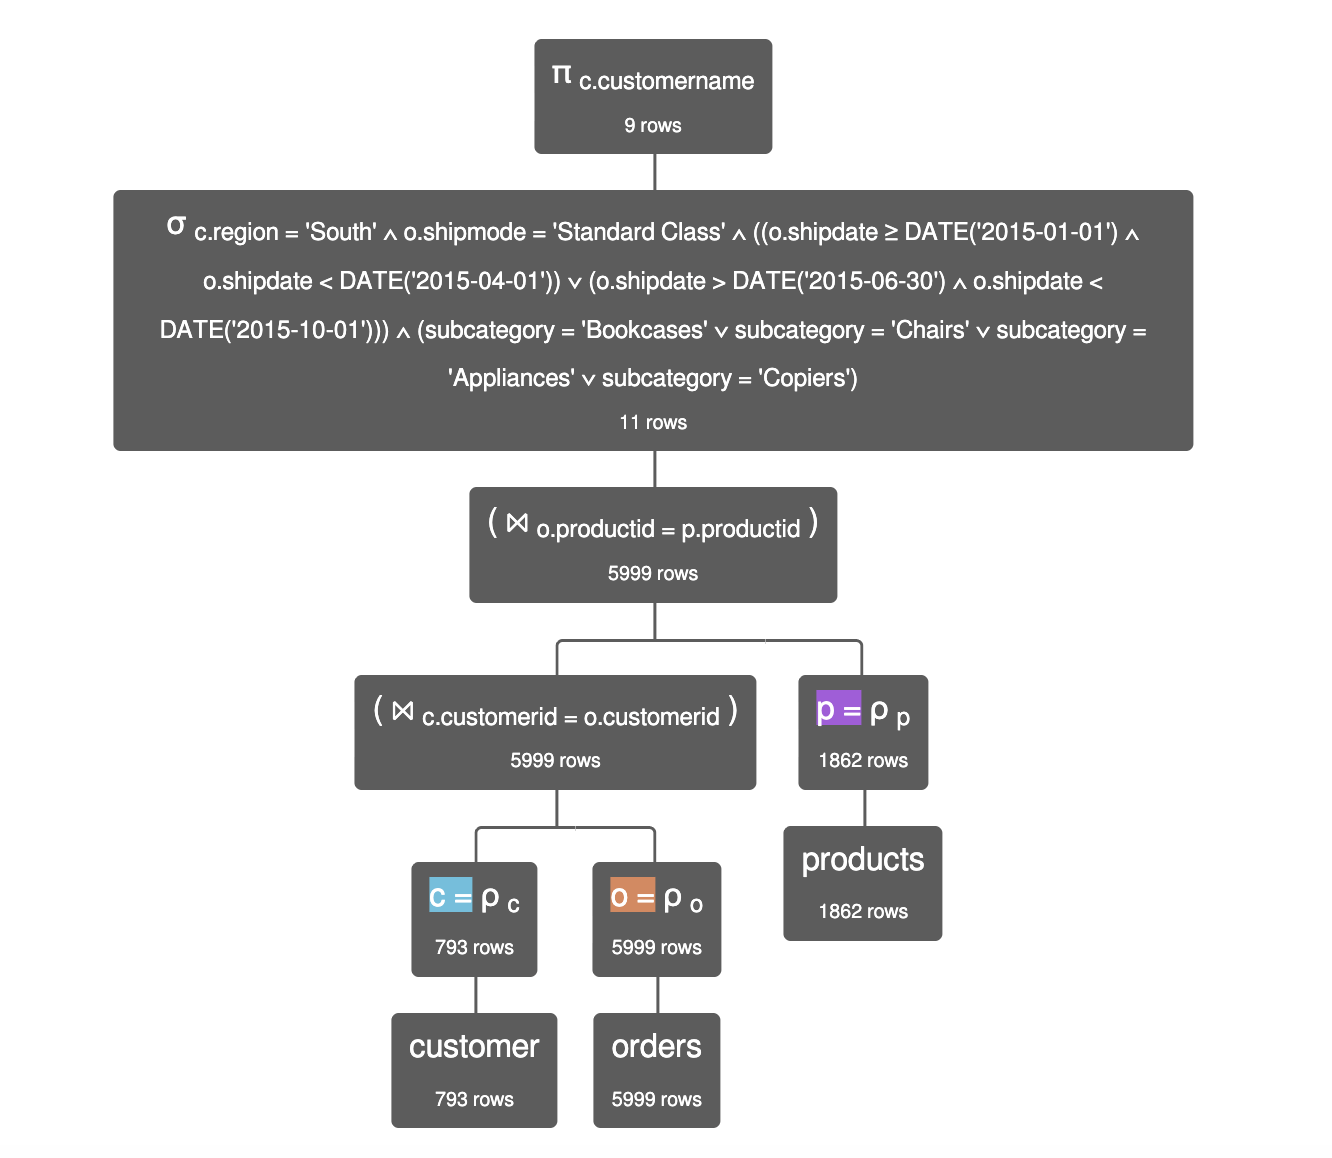
\includegraphics[width=0.8\textwidth]{imagenes/2c(2).png}
\caption{Árbol de consulta.}
\end{figure}

\begin{figure}[h!]
\centering
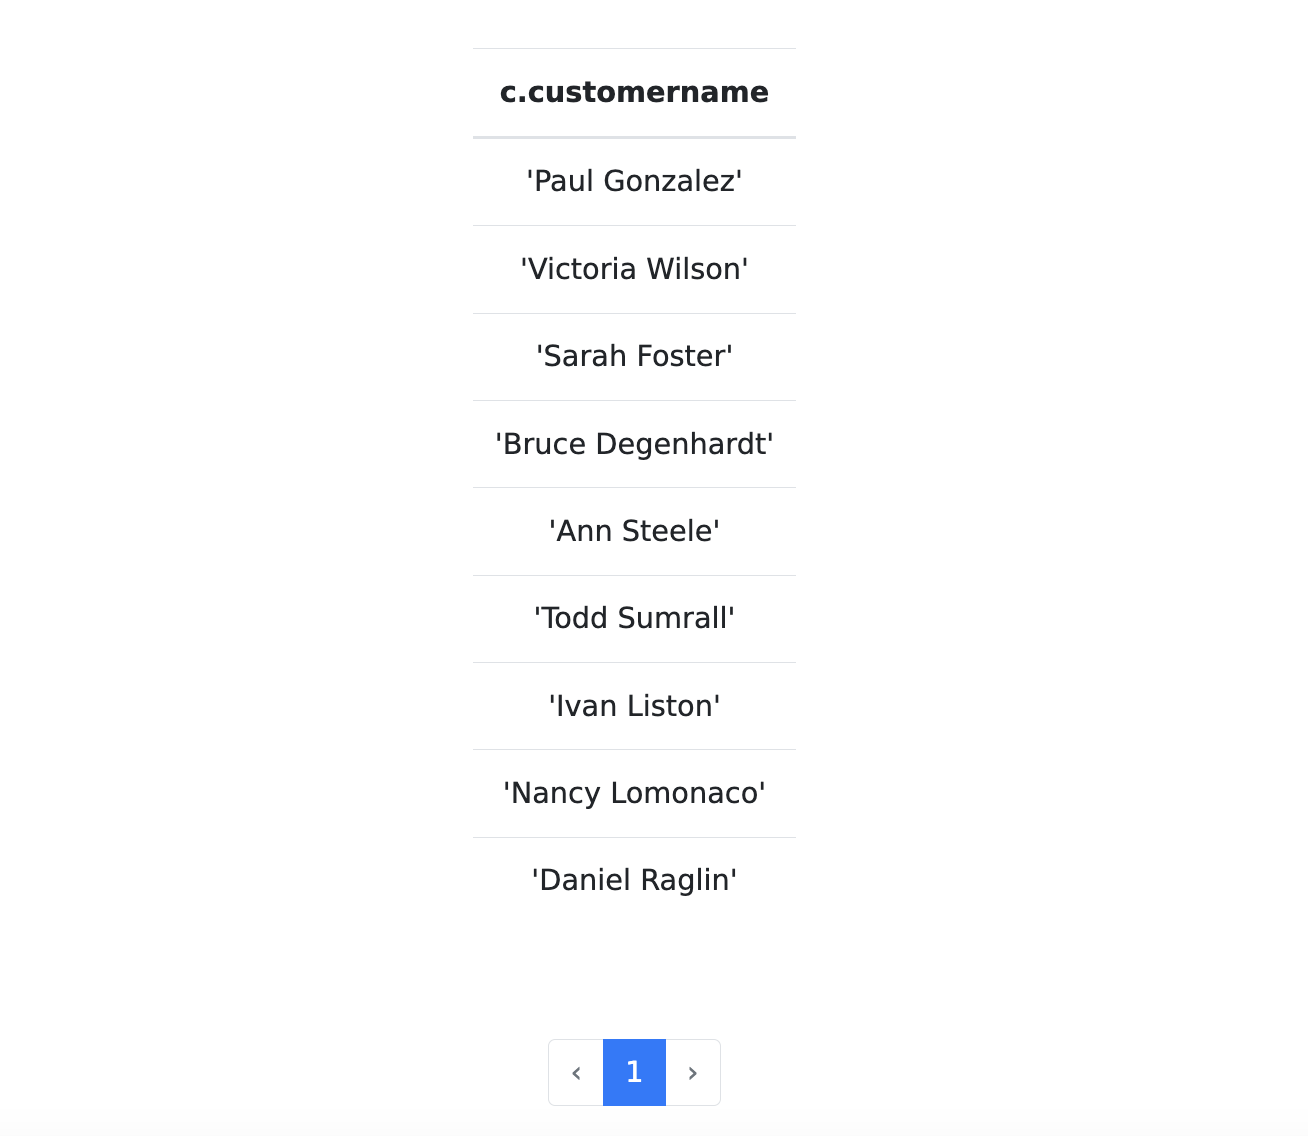
\includegraphics[width=0.6\textwidth]{imagenes/2c(3).png}
\caption{Resultado de consulta.}
\end{figure}

 \subsection*{d. Toda la información de los clientes del segmento Consumer que realizaron una orden con modo de envío Second Class y que no viven en Nevada.}

Primero seleccionamos de \textit{customer} a los clientes del segmento \textit{Consumer} que no viven en \textit{Nevada}. Después seleccionamos de la tabla \textit{orders} las órdenes con modo de envío \textit{Second Class} y proyectamos solamente el id de los clientes que las realizaron. Finalmente, realizamos un join natural entre ambos resultados, para que solamente nos queden los clientes que cumplen todas las condiciones, junto con si información completa.

Expresión:
\begin{equation}
\sigma_{segment = \text{'Consumer'} \, \wedge \, state \neq \text{'Nevada'}}(customer) \bowtie \pi_{customerid}\left(\sigma_{shipmode = \text{'Second Class'}}(orders)\right)
\end{equation}

Resultados obtenidos:

\begin{figure}[h!]
\centering
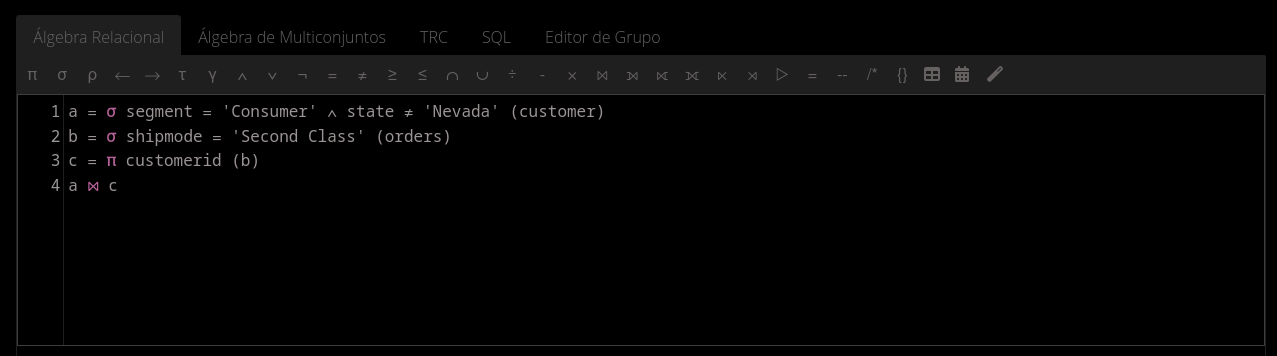
\includegraphics[width=0.8\textwidth]{imagenes/2d(1).png}
\caption{Consulta}
\end{figure}

\begin{figure}[h!]
\centering
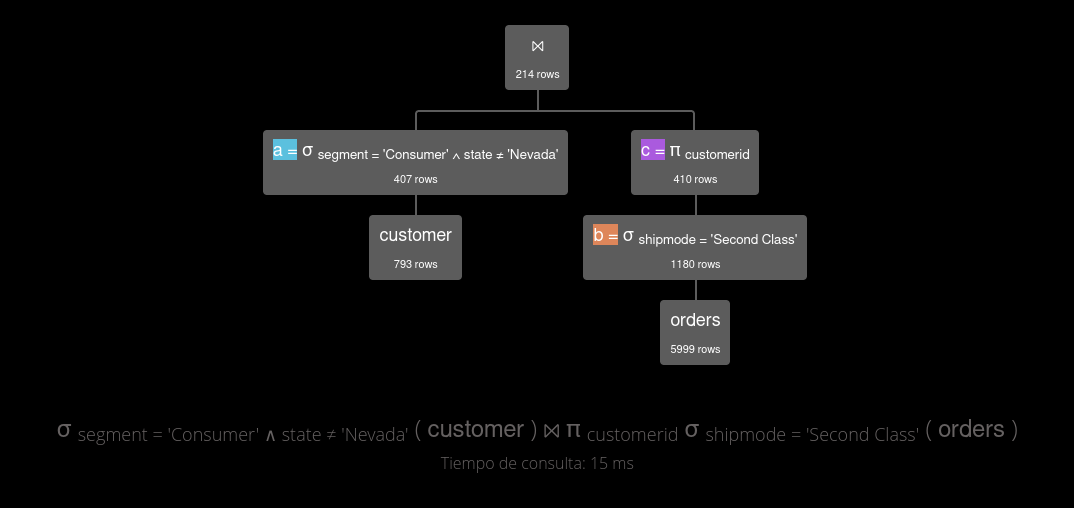
\includegraphics[width=0.8\textwidth]{imagenes/2d(2).png}
\caption{Árbol de consulta.}
\end{figure}

\begin{figure}[h!]
\centering
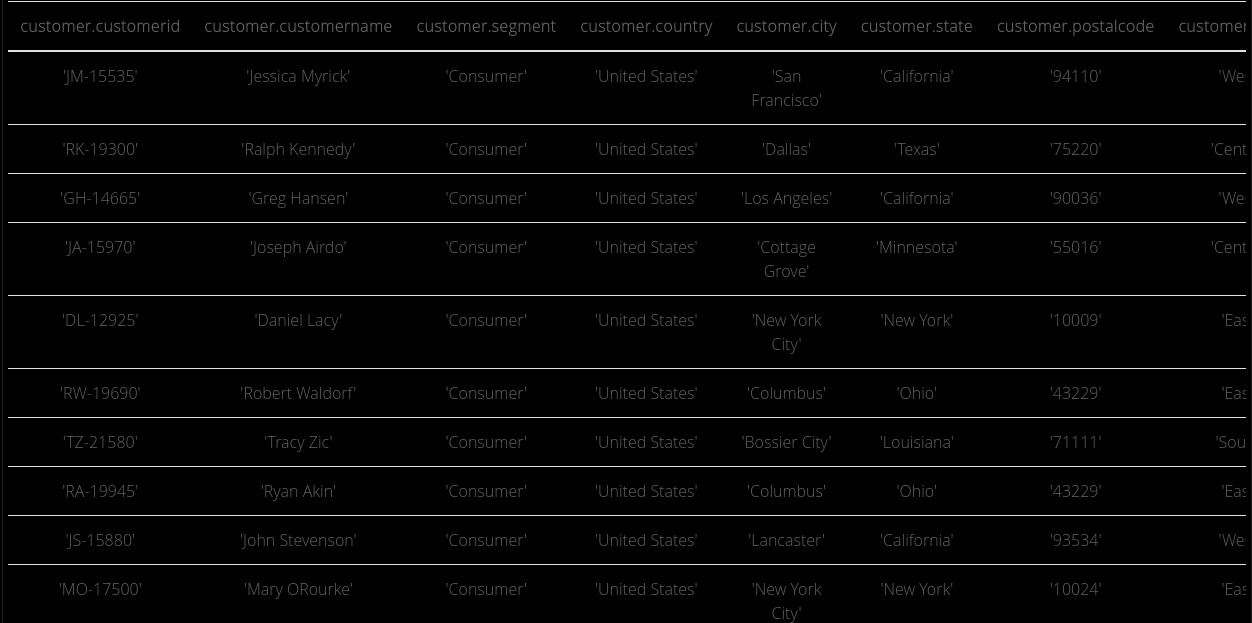
\includegraphics[width=0.8\textwidth]{imagenes/2d(3).png}
\caption{Resultado de consulta.}
\end{figure}
 \subsection*{e. Obtener el estado, segmento y el total de clientes que no han solicitado ninguna orden.}

Primero separaremos a los clientes que tienen una cuenta y no tienen una orden, de los que sí tienen una orden. Posteriormente, obtendremos los atributos de estos clientes y los agruparemos respecto a 'state' y 'segment', contando el número de clientes en cada grupo y colocándolo como una columna llamada 'numclientes'.

Expresión:
\begin{equation}
\gamma_{\text{state}, \text{segment}; \, \text{COUNT}(\text{customerid}) \to \text{numclientes}} \left( \left( \left( \pi_{\text{customerid}}(\text{customer}) - \pi_{\text{customerid}}(\text{orders}) \right) \bowtie \text{customer} \right) \right)
\end{equation}

Resultados Obtenidos:

\begin{figure}[H]
  \centering
  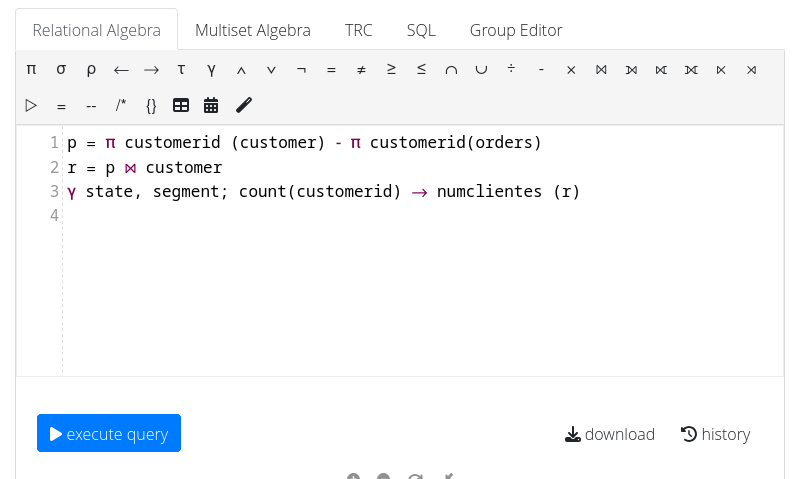
\includegraphics[width=0.7\textwidth]{imagenes/2.e-Query.png}
  \caption{Consulta}
\end{figure}

\begin{figure}[H]
  \centering
  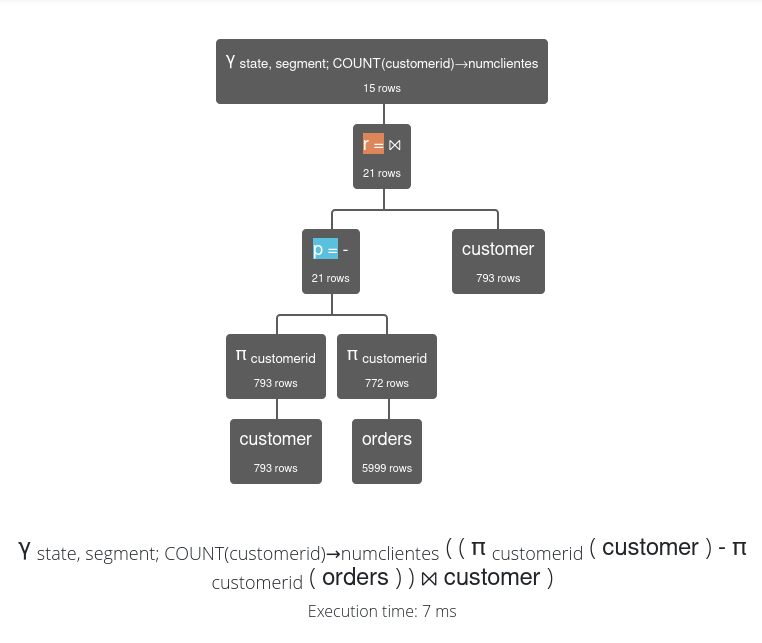
\includegraphics[width=0.7\textwidth]{imagenes/2.e-Three.png}
  \caption{Árbol de consulta.}
\end{figure}

\begin{figure}[H]
  \centering
  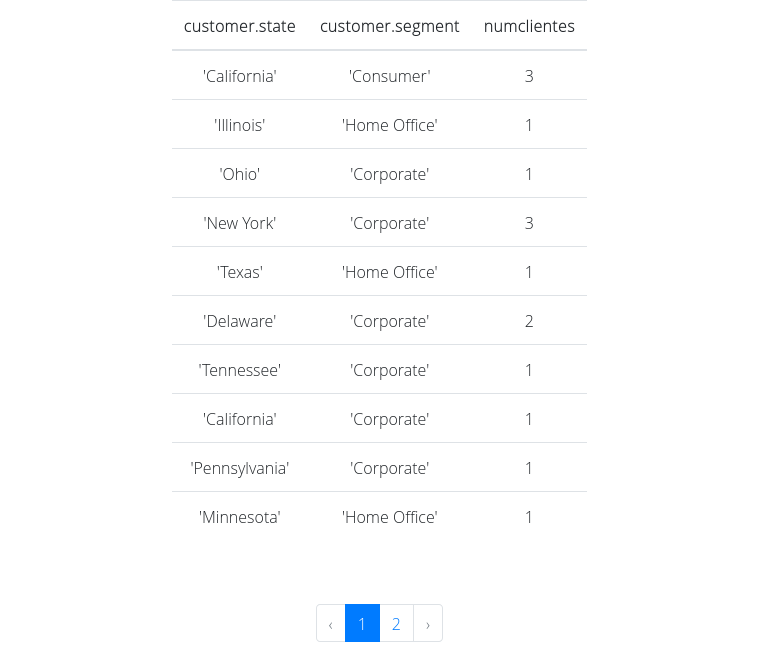
\includegraphics[width=0.7\textwidth]{imagenes/2.e-Tabla.png}
  \caption{Resultado de consulta.}
\end{figure}

 \subsection*{f. Una lista que muestre la región, el estado y el total de clientes que se tienen, considerando que los clientes deben
haber realizado órdenes con al menos 6 productos durante 2016 o 2017. Ordenar la información por región y estado}
Seleccionamos las órdenes de 2016 y 2017, las agrupamos por cliente y orden sumando la cantidad de productos, y nos quedamos con las que tienen al menos 6. Después renombramos la tabla customer como $c$ y realizamos un join con la relación anterior con el id del cliente, de tal forma que cada orden que cumple la condición quede asociada a la información de su cliente. Con ese resultado agrupamos por estado y región, contando los clientes de cada grupo (tot). Finalmente, proyectamos estado, región y total, y renombramos los atributos como edo y reg.\\ \\
Expresión:
\[
\begin{aligned}
&\rho_{edo \leftarrow c.state,\; reg \leftarrow c.region} \\
&\pi_{c.state,\; c.region,\; tot} \\
&\gamma_{c.state,\; c.region;\; \mathrm{COUNT}(customerid) \to tot}\Bigg( \\
&\qquad \rho_{t}\Big( \\
&\qquad\qquad \rho_{clie \leftarrow o.customerid,\; orden \leftarrow o.orderid} \\
&\qquad\qquad \pi_{o.customerid,\; o.orderid,\; productos} \\
&\qquad\qquad \sigma_{productos > 5} \\
&\qquad\qquad \gamma_{o.customerid,\; o.orderid;\; \mathrm{SUM}(o.quantity) \to productos} \\
&\qquad\qquad \sigma_{\substack{
    o.orderdate \geq \text{DATE('2016-01-01')} \; \\
    \land\; o.orderdate < \text{DATE('2018-01-01')}
  }} \\
&\qquad\qquad \rho_{o}(orders) \\
&\qquad\Big) \\
&\qquad \bowtie_{t.clie = c.customerid} \rho_{c}(customer) \\
&\Bigg)
\end{aligned}
\]
\newpage
Resultados obtenidos:

\begin{figure}[h!]
\centering
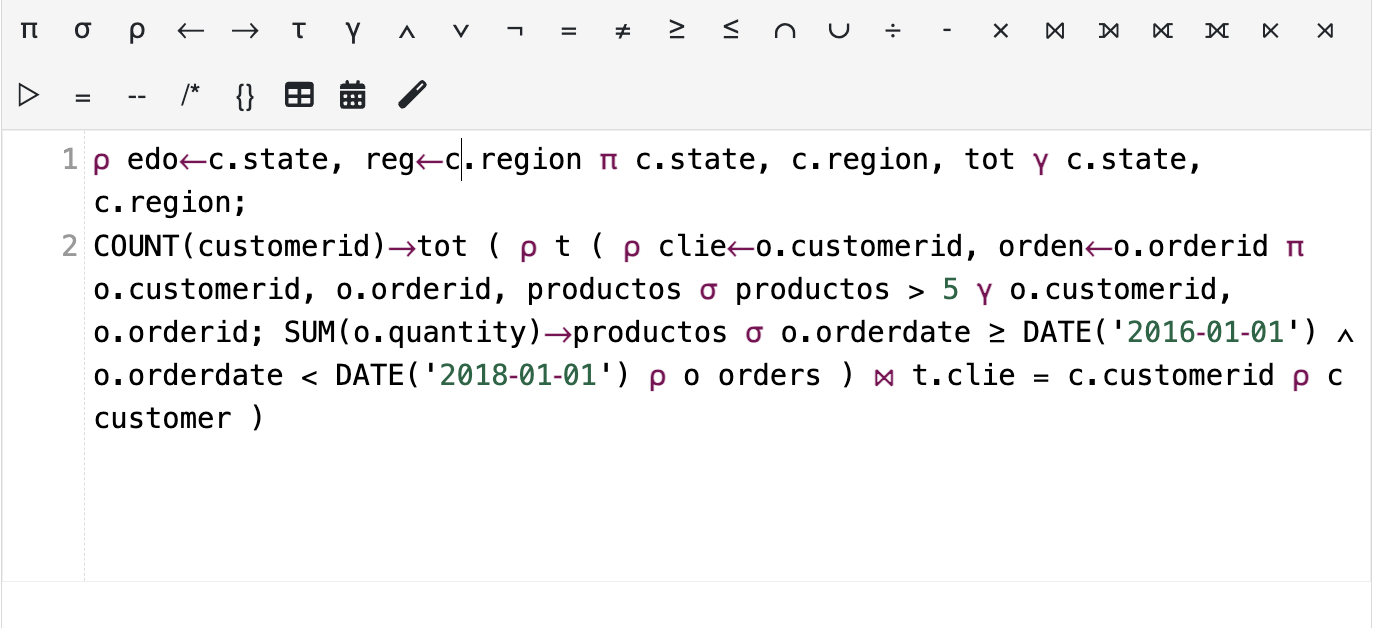
\includegraphics[width=0.8\textwidth]{imagenes/2f(1).png}
\caption{Consulta}
\end{figure}

\begin{figure}[h!]
\centering
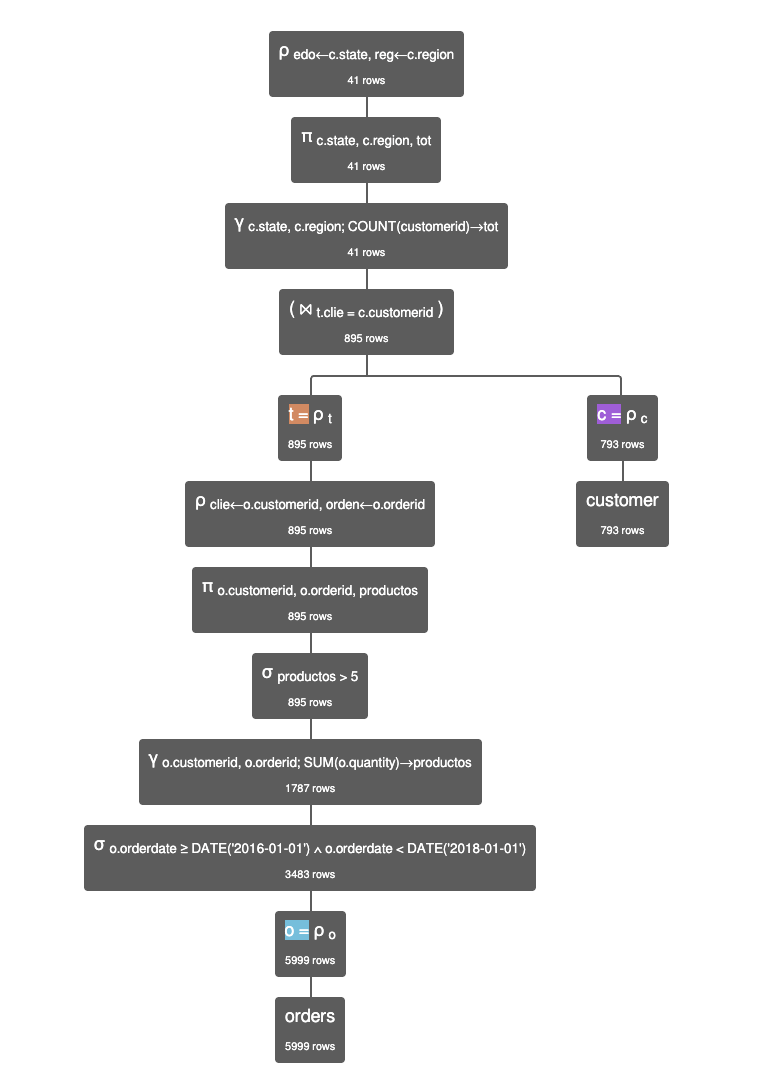
\includegraphics[width=0.8\textwidth]{imagenes/2f(2).png}
\caption{Árbol de consulta.}
\end{figure}

\begin{figure}[h!]
\centering
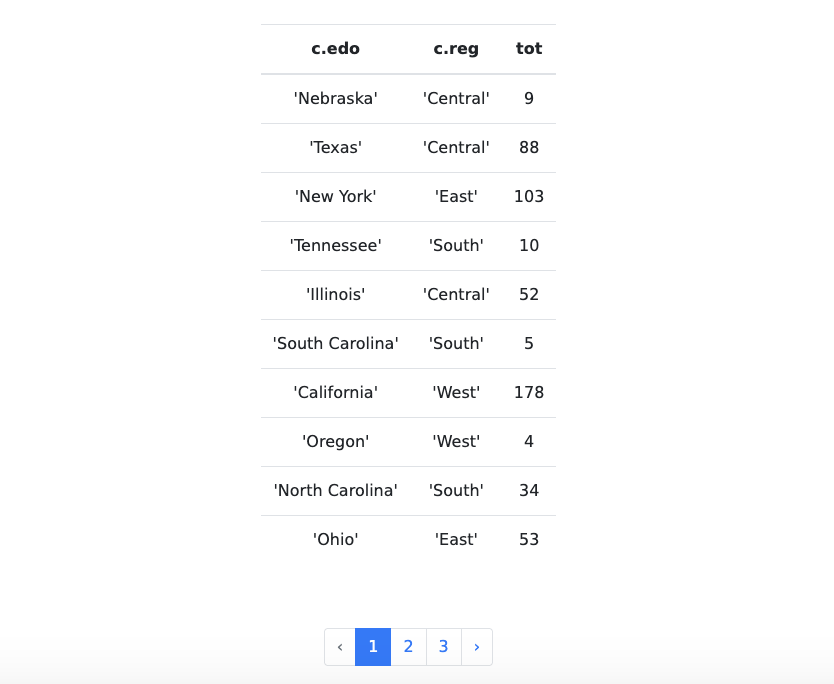
\includegraphics[width=0.6\textwidth]{imagenes/2f(3).png}
\caption{Resultado de consulta.}
\end{figure}
 \subsection*{g. Obtener el modo de envío y categoría que más productos ha vendido.}

Primero realizamos un join natural entre la tabla \textit{orders} y la tabla \textit{products} (comparten productid) para poder asociar las cantidades (\textit{quantity}), los modos de envío (\textit{shipmode}) y las categorías (\textit{category}). Después, aplicamos una operación $\gamma$ para agrupar por \textit{shipmode} y \textit{category}, y le aplicamos la función de agregación SUM a la cantidad de productos (\textit{quantity}), nombrando este valor agregado como \textit{TotalQty}. Llamaremos a esta relación $T$. Luego, sobre $T$ calculamos el valor máximo de estos totales (\textit{MaxQty}), realizando una nueva agrupación. A este resultado lo llamaremos $T_{max}$. Finalmente, cruzamos $T$ con $T_{max}$ (haciendo match donde \textit{TotalQty} sea igual a \textit{MaxQty}) y proyectamos únicamente los atributos \textit{shipmode} y \textit{category}.

Expresión:
\begin{equation}
\begin{split}
T &= \gamma_{shipmode,\, category;\, \text{SUM}(quantity) \rightarrow TotalQty}(orders \bowtie products) \\
T_{max} &= \gamma_{\text{MAX}(TotalQty) \rightarrow MaxQty}(T) \\
\text{Resultado} &= \pi_{shipmode,\, category}(T \bowtie_{TotalQty = MaxQty} T_{max})
\end{split}
\end{equation}

Resultados obtenidos:

\begin{figure}[h!]
\centering
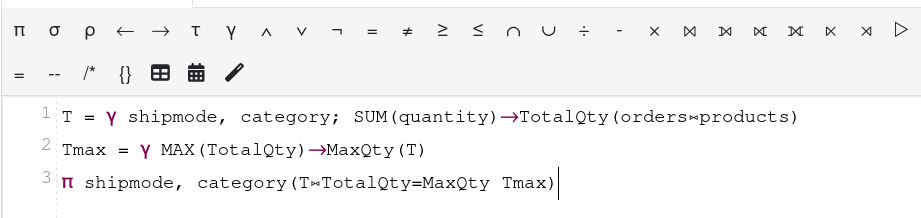
\includegraphics[width=0.8\textwidth]{imagenes/2g(1).png}
\caption{Consulta 2g.}
\end{figure}

\begin{figure}[h!]
\centering
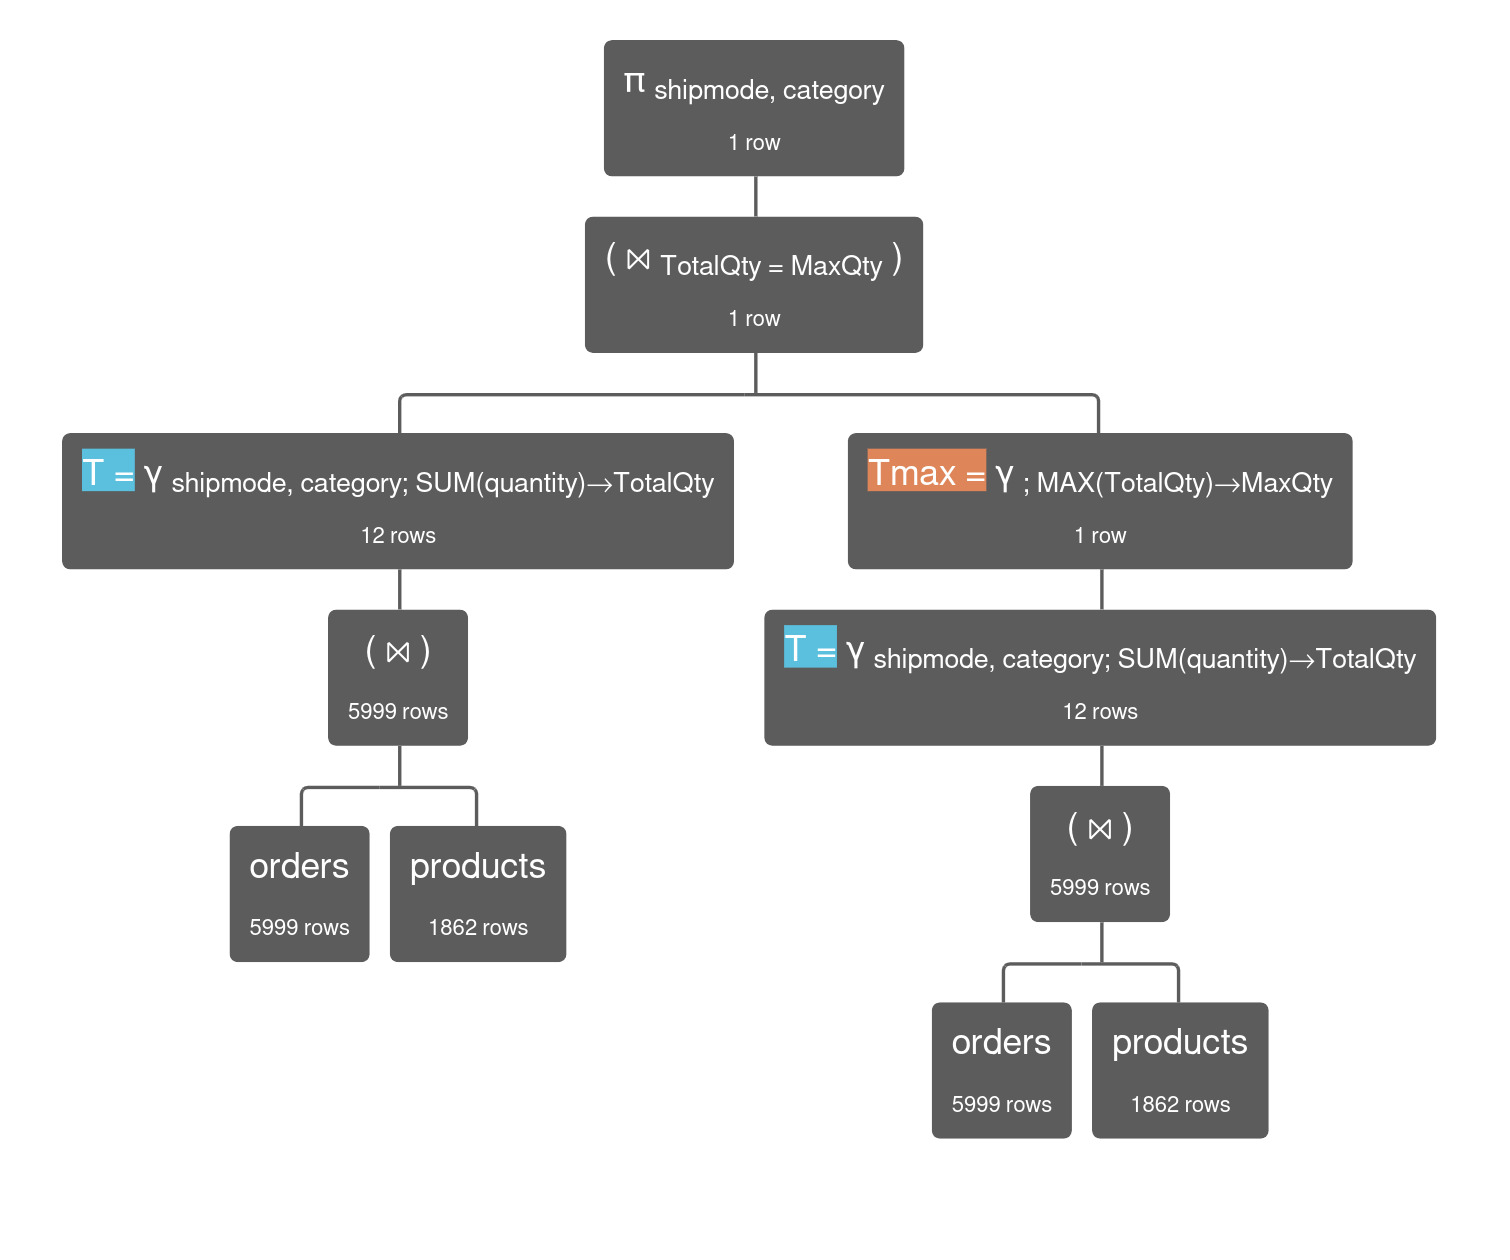
\includegraphics[width=0.8\textwidth]{imagenes/2g(2).png}
\caption{Árbol de consulta 2g.}
\end{figure}

\begin{figure}[h!]
\centering
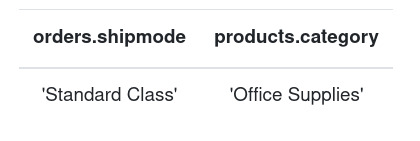
\includegraphics[width=0.8\textwidth]{imagenes/2g(3).png}
\caption{Resultado de consulta 2g.}
\end{figure}

 \subsection*{h. Una lista con la venta promedio, venta total, mayor venta, menor venta, y total de órdenes, por región, estado y ciudad. La venta promedio debe estar entre \$ 900 y \$1,500.}

Para este ejercicio, primero obtendremos una tabla con los elementos necesarios para realizar los cálculos. Para esto, por cada región, estado y ciudad, necesitamos conocer cada orden realizada y el valor de la venta.

Posteriormente, podemos usar la tabla del paso anterior y agrupar sus tuplas en base a la región, estado y ciudad, agregando además nuevas columnas para los valores que podemos calcular a partir de las órdenes y los valores realizados. 
\begin{itemize}
    \item Para el promedio usamos avg() sobre las ventas y la columna 'promedio'
    \item Para el máximo usamos max() sobre las ventas y la columna 'ventamaxima'
    \item Para el mínimo usamos min() sobre las ventas y la columna 'ventaminima' 
    \item Para la cantidad de órdenes, usamos count() sobre orderid y la columna 'totalordenes'
\end{itemize}

Finalmente, usamos la tabla anterior para escoger solo aquellos elementos en los que el promedio está entre \$ 900 y \$1500

Así, obtenemos la expresión:
\begin{equation}
\begin{split}
&\sigma_{\text{promedio} \geq 900 \land \text{promedio} \leq 1500} \Biggl( \gamma_{\substack{\text{region, state, city}; \\ \text{AVG(venta)} \to \text{promedio}, \text{SUM(venta)} \to \text{ventas}, \\ \text{MAX(venta)} \to \text{ventamaxima}, \text{MIN(venta)} \to \text{ventaminima}, \\ \text{COUNT(orderid)} \to \text{totalordenes}}} \\
&\Biggl( \left( \pi_{\substack{\text{customerid, orderid,} \\ \text{venta} \leftarrow \text{quantity} * \text{price}}} ( \text{orders} \bowtie \text{products} ) \right) \bowtie \text{customer} \Biggr) \Biggr) 
\end{split}
\end{equation}

Resultados obtenidos:

\begin{figure}[H]
    \centering
    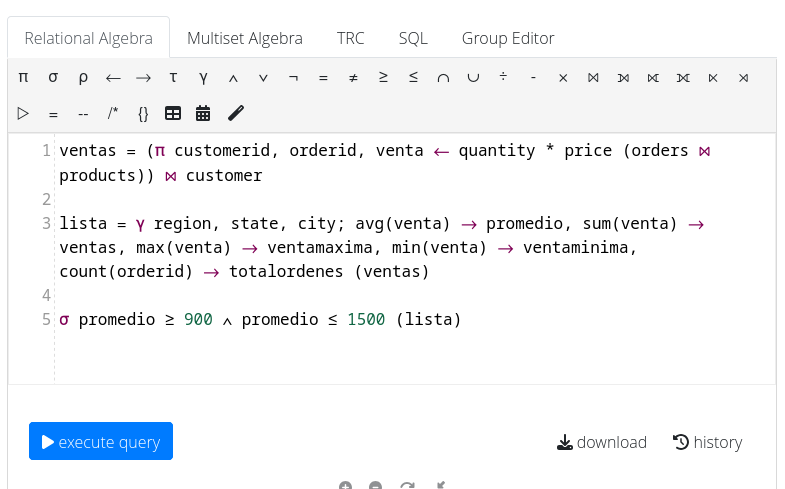
\includegraphics[width=0.7\textwidth]{imagenes/2.h-Query.png}
    \caption{Consulta}
\end{figure}

\begin{figure}[H]
    \centering
  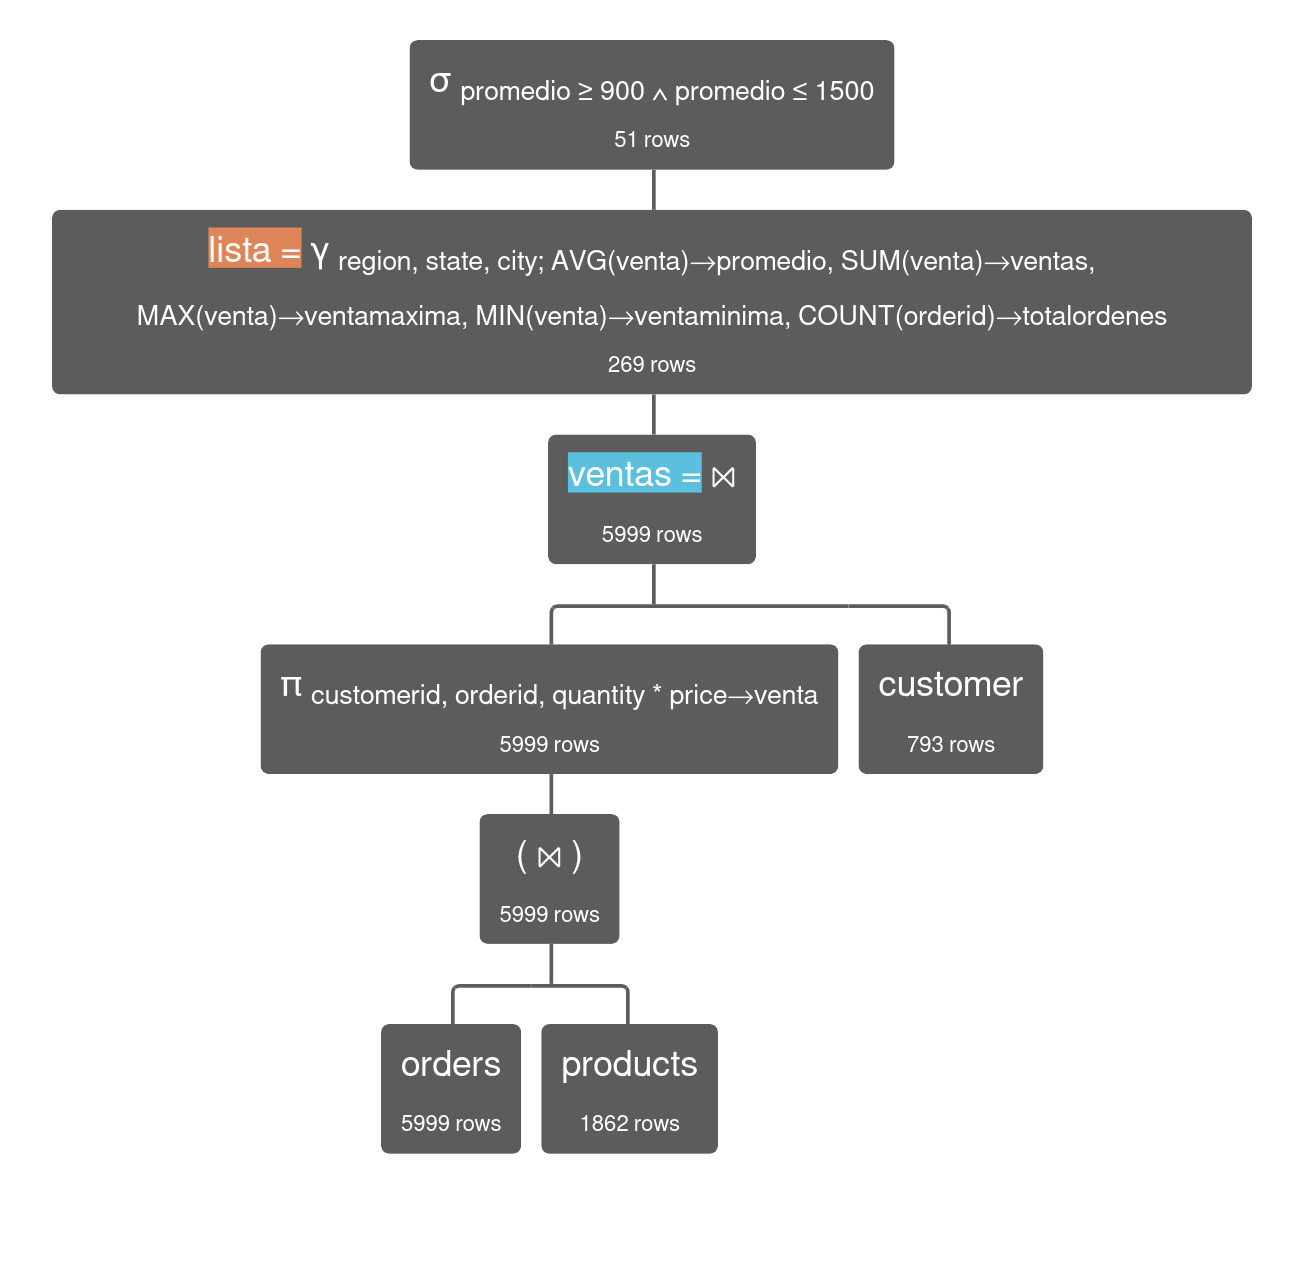
\includegraphics[width=0.7\textwidth]{imagenes/2.h-Three.png}
    \caption{Árbol de consulta.}
\end{figure}

    
\begin{figure}[H]
    \centering
  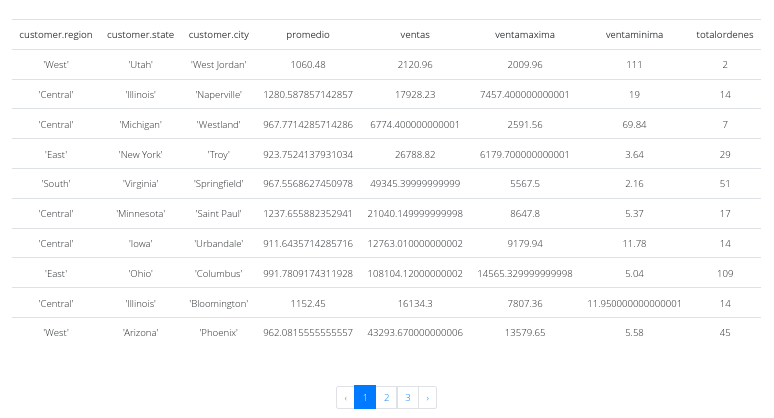
\includegraphics[width=0.7\textwidth]{imagenes/2.h-Tabla.png}
    \caption{Resultado de consulta.}
\end{figure}

 \subsection*{i. El estado que ha realizado la menor cantidad de órdenes. Se debe mostrar también el total de ordenes que haya entregado.}
\addcontentsline{toc}{subsection}{i.}

Primero, se realiza un JOIN entre \texttt{customer} y \texttt{orders} con el ID de cliente de ambas tablas. Luego, los registros se agrupan por el estado de vivienda de los clientes, y se realiza un conteo por id (que, como es único y no nulo, es en escencia un conteo de filas), lo que realiza un conteo de registros por estado y, finalmente, el resultado se ordena de forma descendente.

La notación en álgebra lineal no permite formular nativamente la operación \texttt{LIMIT}, pero se puede observar, según el primer registro de la columna, que el estado con más pedidos es California, con un registro total de 1200.

Expresión:
\begin{itemize}[nosep]
\item [\ ] $\tau_{totalorders\ desc}$
\item [\ ] $($
        \begin{itemize}
            \item [\ ] $\gamma_{customer.state;\ count(orders.orderid)\rightarrow totalorders}$
            $($
            \begin{itemize}
                \item [\ ] $customer$
                    \begin{itemize}
                        \item [\ ] $\bowtie_{customer.customerid=orders.customerid}$
                    \end{itemize}
                \item [\ ] $orders$
            \end{itemize}
            $)$
        \end{itemize}
    $)$
\end{itemize}


Resultados obtenidos:

\begin{figure}[h!]
\centering
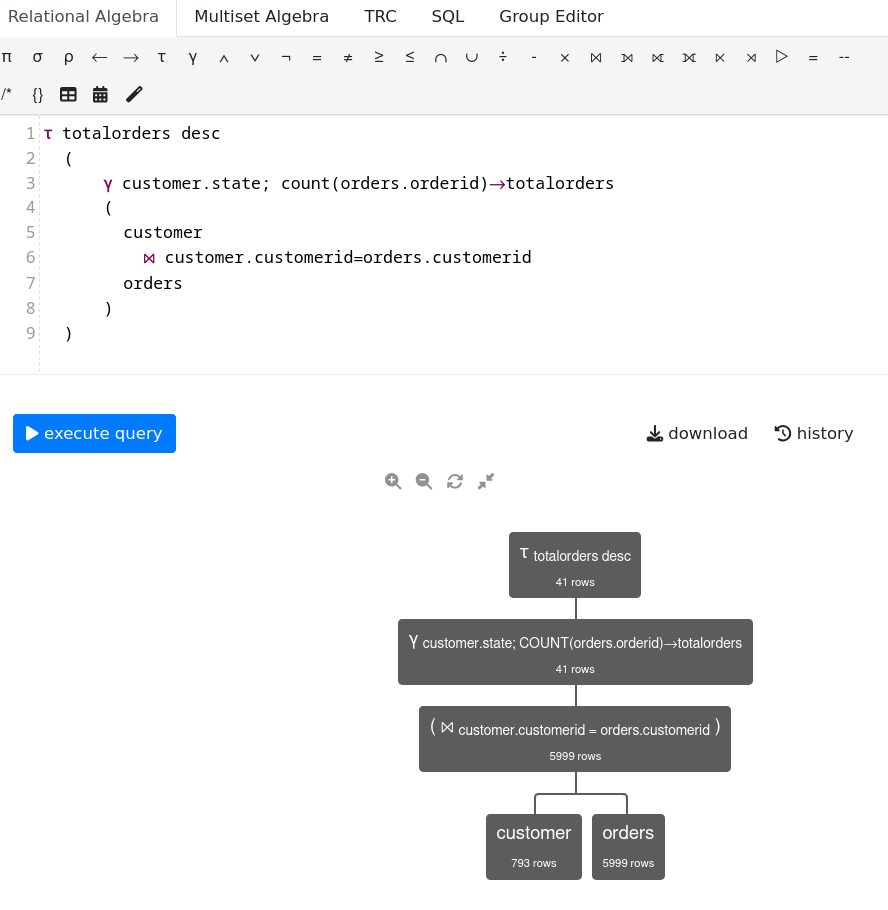
\includegraphics[width=0.8\textwidth]{imagenes/result2I1.png}
\caption{Consulta y árbol generado.}
\end{figure}

\begin{figure}[h!]
\centering
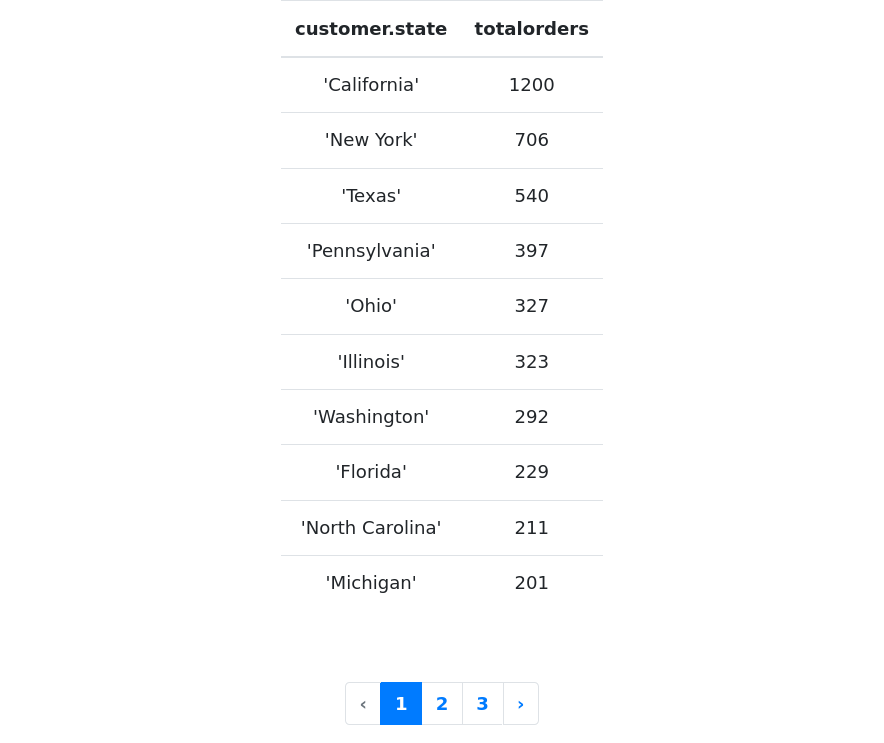
\includegraphics[width=0.8\textwidth]{imagenes/result2I2.png}
\caption{Resultado de consulta.}
\end{figure}
 \subsection*{j. La información del cliente que más órdenes haya efectuado. Mostrar el número de órdenes que ha realizado.}

Primero agrupamos la tabla \textit{orders} por \textit{customerid} para contar el total de órdenes efectuadas usando la función COUNT sobre \textit{orderid}. Nombramos este agregado como \textit{numorders} y llamaremos a esta operación $T$. Después, buscamos el valor máximo de órdenes registradas aplicando la función de agregación MAX sobre \textit{numorders} en una nueva agrupación. Este paso se guarda como $T_{max}$. Hacemos un join de $T$ y $T_{max}$ indicando en la condición $\theta$ que \textit{numorders} debe ser igual a \textit{MaxOrders}, filtrando así únicamente el o los IDs de cliente con la máxima participación. Por último, aplicamos un join natural con la tabla \textit{customer} para obtener toda la información del cliente ganador, y usamos una proyección para presentar todos sus atributos junto con la columna adicional \textit{numorders}.

Expresión:
\begin{equation}
\begin{split}
T &= \gamma_{customerid;\, \text{COUNT}(orderid) \rightarrow numorders}(orders) \\
T_{max} &= \gamma_{\text{MAX}(numorders) \rightarrow MaxOrders}(T) \\
\text{Resultado} &= \pi_{customer.*,\, numorders} (customer \bowtie (T \bowtie_{numorders = MaxOrders} T_{max}))
\end{split}
\end{equation}

Resultados obtenidos:

\begin{figure}[h!]
\centering
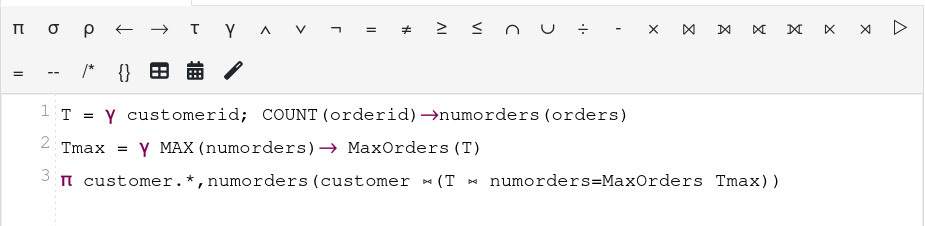
\includegraphics[width=0.8\textwidth]{imagenes/2j(1).png}
\caption{Consulta 2j.}
\end{figure}

\begin{figure}[h!]
\centering
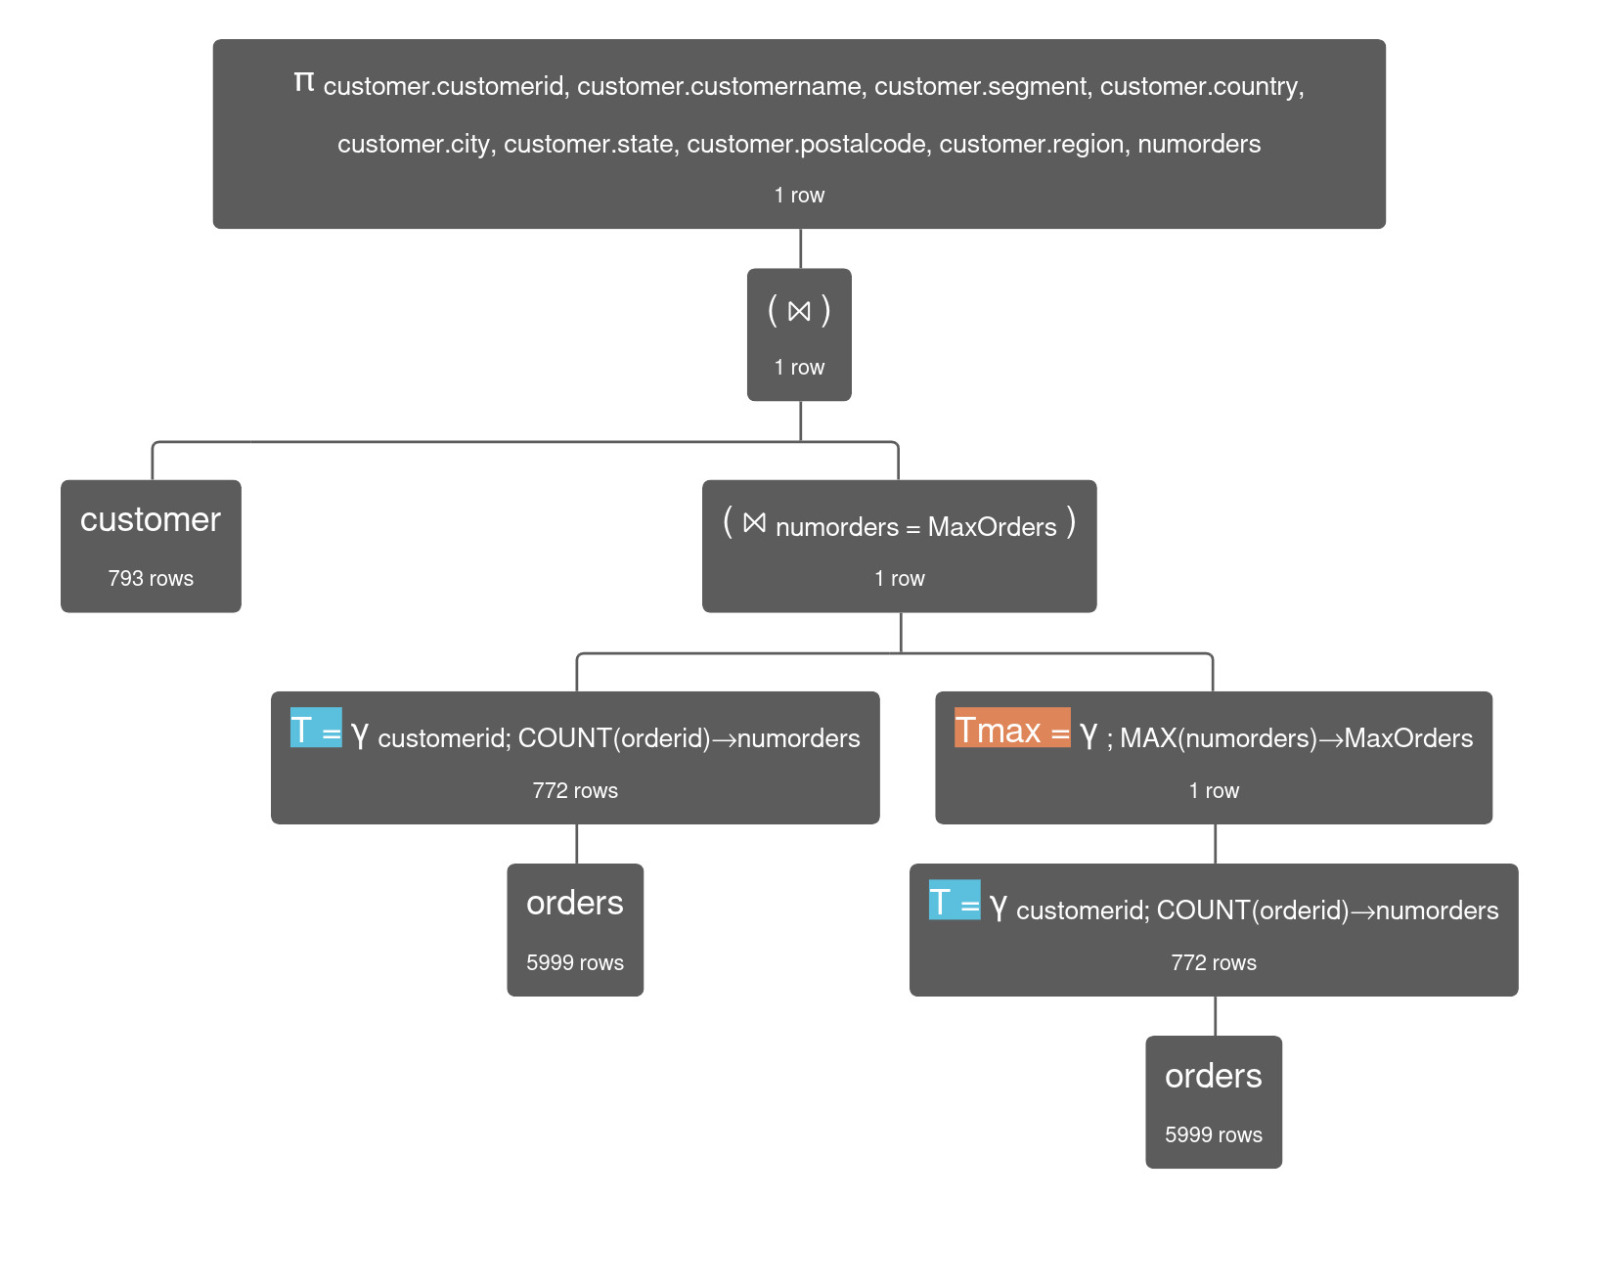
\includegraphics[width=0.8\textwidth]{imagenes/2j(2).png}
\caption{Árbol de consulta 2j.}
\end{figure}

\begin{figure}[h!]
\centering
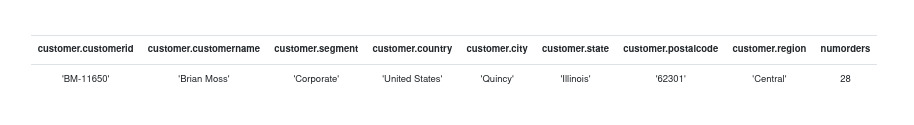
\includegraphics[width=0.8\textwidth]{imagenes/2j(3).png}
\caption{Resultado de consulta 2j.}
\end{figure}


 % Ejercicio 3
 \subsection*{a. Borrar toda la información del cliente Paul Stevenson.}
Para esto usaremos la diferencia de conjuntos. Primero ubicaremos toda la información de Paul Stevenson en la tabla customers y posteriormente eliminaremos de la tabla.

Esto lo realizamos con la expresion:
\begin{equation}
\text{customer} - \sigma_{\text{customername} = \text{'Paul Stevenson'}} ( \text{customer} )
\end{equation}

Resultados obtenidos:
\begin{figure}[H]
  \centering
  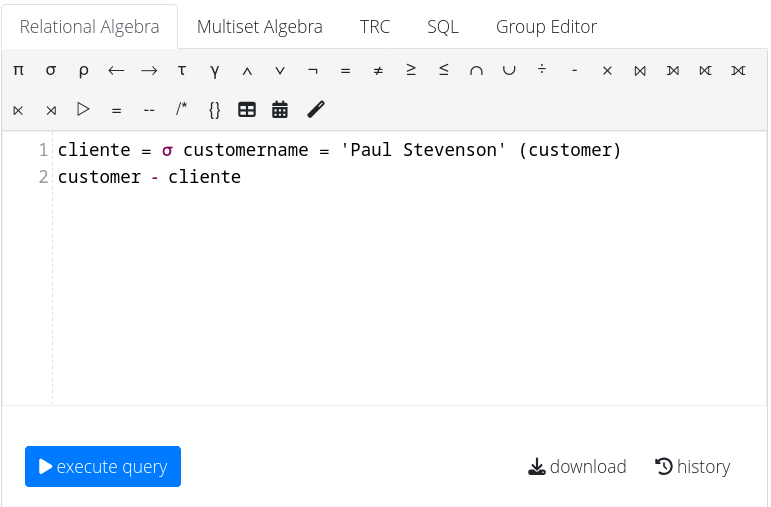
\includegraphics[width=0.7\textwidth]{imagenes/3.a-Query.png}
  \caption{Consulta}
\end{figure}

\begin{figure}[H]
  \centering
  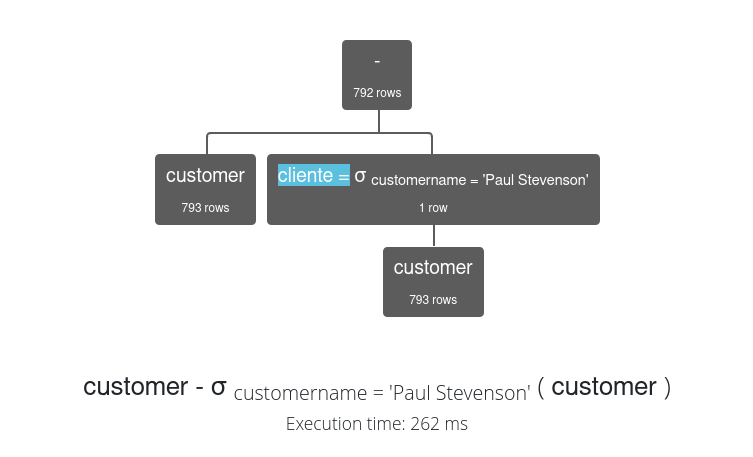
\includegraphics[width=0.7\textwidth]{imagenes/3.a-Three.png}
  \caption{Árbol de consulta.}
  \end{figure}
  
  \begin{figure}[H]
    \centering
    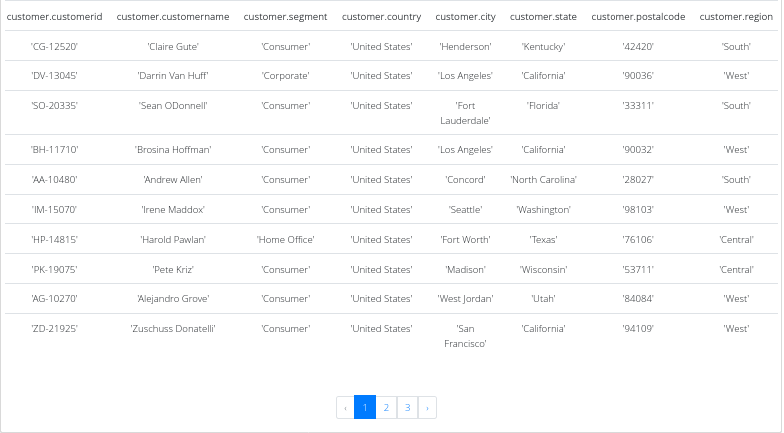
\includegraphics[width=0.7\textwidth]{imagenes/3.a-Tabla.png}
    \caption{Resultado de consulta.}
  \end{figure}

 \subsection*{b. Borrar todas las órdenes de la ciudad Utah que tengan artículos de la subctegoría Tables.}
\subsubsection*{Desarrollo de operación.}
Primero, se hizo un JOIN de órdenes y productos conforme al atributo de \texttt{productid} que comparten, filtrando los productos en la subcategoría `\textit{Tables}', y se conservó solo la parte de órdenes (obteniendo un subconjunto), esto bajo el nombre de \texttt{r}.

Después, se hizo un JOIN de \texttt{r} y clientes, esto conforme al atributo de \texttt{customerid} que comparten, filtrando los clientes con vivienda en Utah, y se conservó solo la parte de órdenes (obteniendo un subconjunto), esto bajo el nombre de \texttt{s}.

Así, se tiene que \texttt{s} es la parte de \texttt{orders} con productos asociados con subcategoría `\textit{Tables}' y clientes asociados con vivienda en Utah.

Finalmente, basta con hacer la consulta con la resta de \texttt{s} a \texttt{orders} para producir la eliminación.

\addcontentsline{toc}{subsection}{b.}

Expresion:
\begin{itemize}[nosep]
\item [\ ] $r =$
    \begin{itemize}
    \item [\ ] $\pi_{orders.*}$
    \item [\ ] $($
        \begin{itemize}
            \item [\ ] $\sigma_{products.subcategory = 'Tables'}$
                \begin{itemize}
                    \item [\ ] $(orders$
                        \begin{itemize}
                            \item [\ ] $\bowtie_{orders.productid = products.productid}$
                        \end{itemize}
                    $products)$
                \end{itemize}
        \end{itemize}
    $)$
\end{itemize}
\item [\ ] $	$
$s =$
\begin{itemize}
\item [\ ] $\pi_{orders.*}$
\item [\ ] $($
    \begin{itemize}
    \item [\ ] $\sigma_{customer.state = 'Utah'}$
            \begin{itemize}
                \item [\ ] $(customer$
                    \begin{itemize}
                        \item [\ ] $\bowtie_{customer.customerid = r.customerid}$
                    \end{itemize}
                $r)$
            \end{itemize}
\end{itemize}
$)$
\end{itemize}
$	$
$orders-s$

\end{itemize}
Resultados obtenidos:
\begin{figure}[h!]
\centering
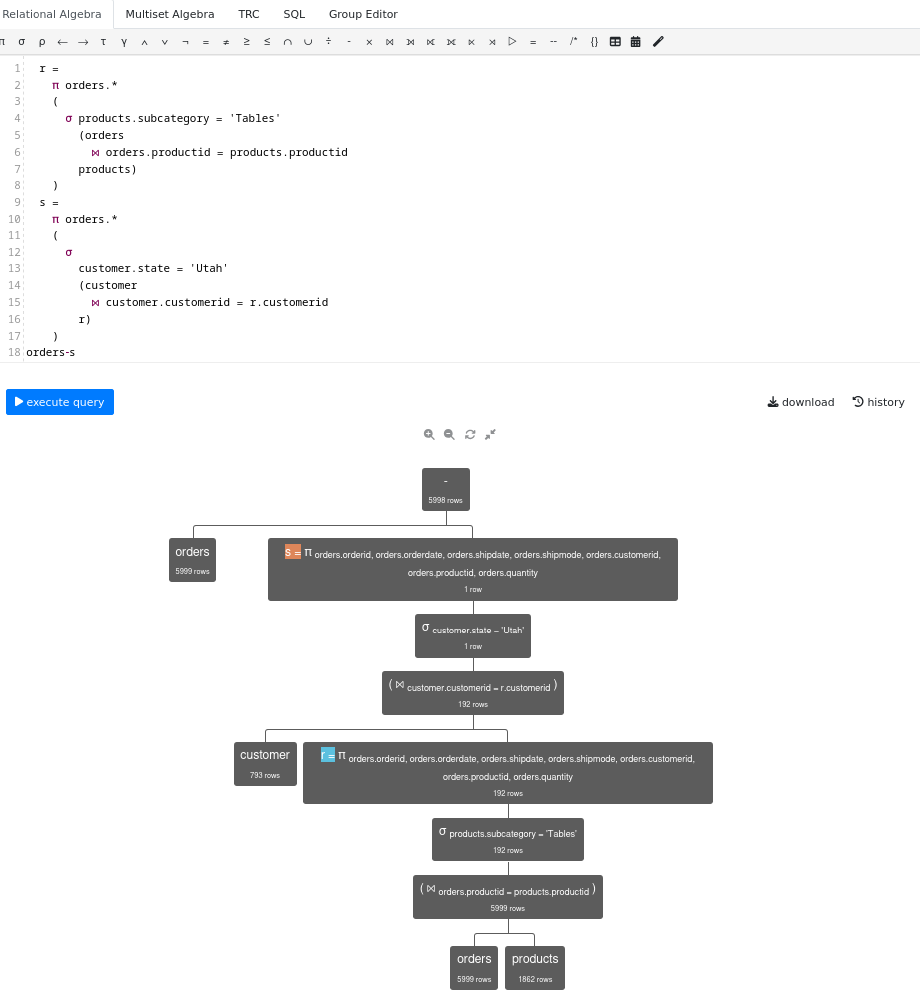
\includegraphics[width=0.8\textwidth]{imagenes/result3B1.png}
\caption{Consulta y árbol generado.}
\end{figure}

\begin{figure}[h!]
\centering
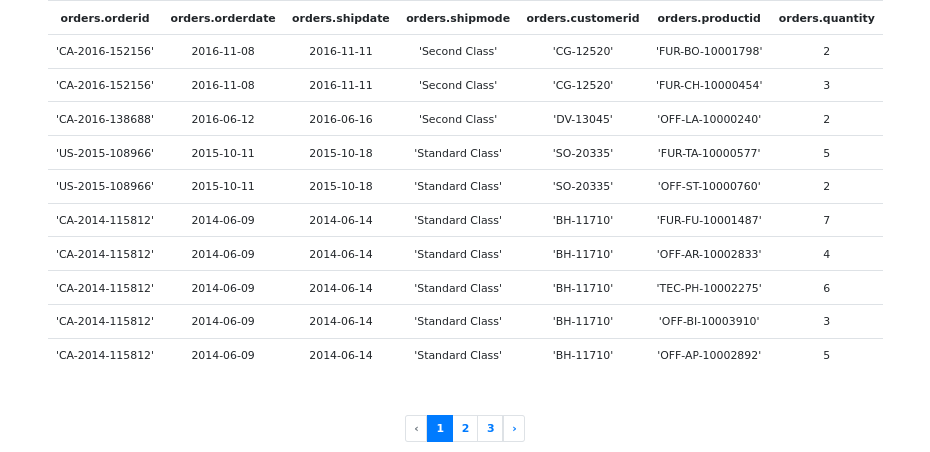
\includegraphics[width=0.8\textwidth]{imagenes/result3B2.png}
\caption{Resultado generado.}
\end{figure}

 \subsection*{c. La clienta Lena Cacioppo compró un producto de cada subcategoría de Furniture. Deberás elegir los productos que desees e indicar como parte de esta consulta, la información que se agregará en cada caso.}

Primero seleccionamos los productos de la categoría Furniture y los agrupamos por subcategoría, eligiendo en cada una el producto con el id más alto, para obtener un producto por subcategoría. Renombramos este resultado como muebles.\\ \\
Usando una proyección, agregamos a cada producto los datos fijos de la compra: el id de la clienta Lena Cacioppo (\textit{LC-16870}), el id de la orden (\textit{US-2026-169552}), la fecha del pedido (30 de octubre de 2026), la fecha de envío (29 de noviembre de 2026), el modo de envío (\textit{Second Class}) y la cantidad (1).

Expresión:
\[
\begin{aligned}
&\pi_{\text{'LC-16870'} \to cliente,\; pid,\; \text{'US-2026-169552'} \to orden,\; \text{DATE('2026-10-29')} \to pedidoen,} \\
&\quad{}_{\text{DATE('2026-11-29')} \to enviadoen,\; \text{'Second Class'} \to modoenvio,\; 1 \to cantidad}\Bigg( \\
&\qquad \rho_{muebles}\Big( \qquad\qquad \pi_{pid} \\
&\hspace{2.2 cm}\qquad\qquad \gamma_{subcategory;\; \mathrm{MAX}(productid) \to pid} \\
&\hspace{2.2 cm} \qquad\qquad \sigma_{category = \text{'Furniture'}}\; products \qquad\Big)\Bigg)\\
\end{aligned}
\]
Resultados obtenidos:

\begin{figure}[h!]
\centering
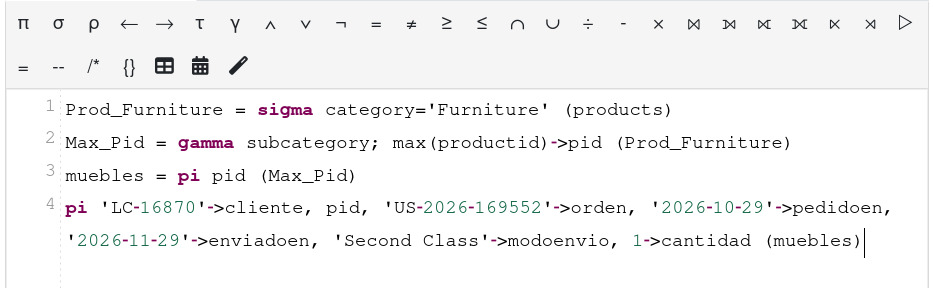
\includegraphics[width=0.9\textwidth]{imagenes/3c(1).png}
\caption{Consulta}
\end{figure}

\begin{figure}[h!]
\centering
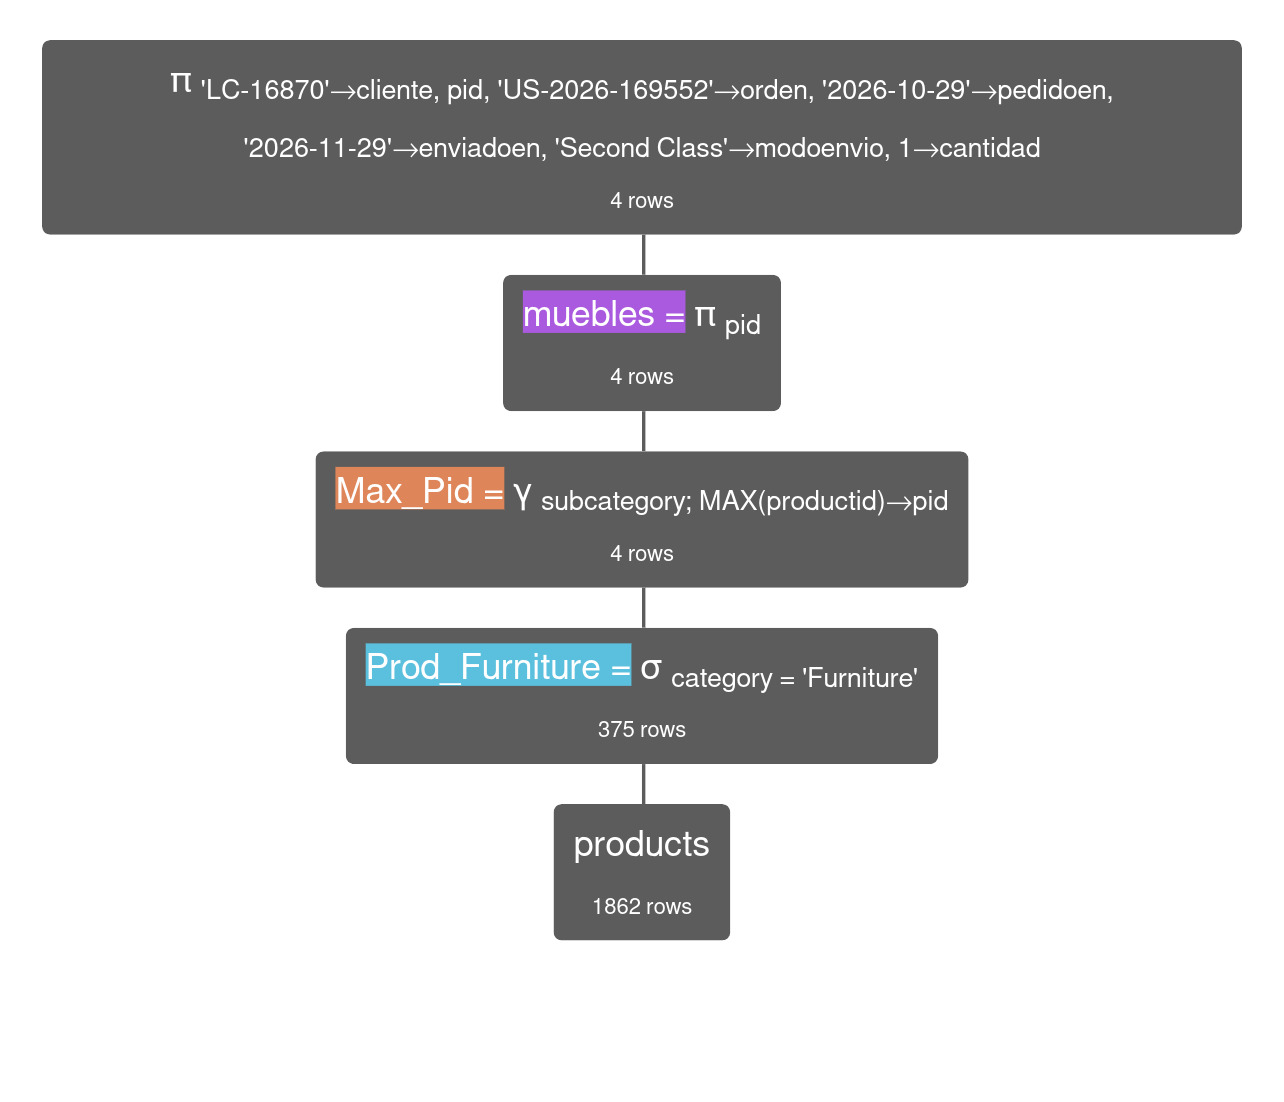
\includegraphics[width=0.72\textwidth]{imagenes/3c(2).png}
\caption{Árbol de consulta.}
\end{figure}

\begin{figure}[h!]
\centering
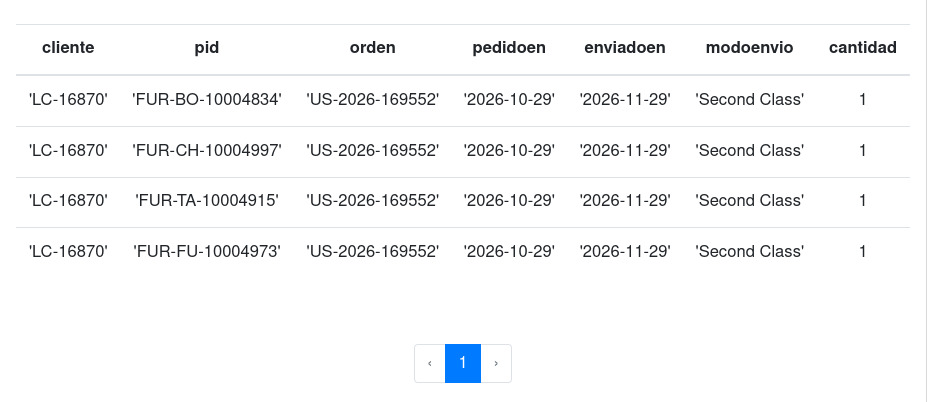
\includegraphics[width=0.8\textwidth]{imagenes/3c(3).png}
\caption{Resultado de consulta.}
\end{figure}

 \subsection*{d. Aumentar los precios de productos de la subcategoría Phones en un 8\%.}
Primero seleccionamos de la tabla \textit{products} los de la subcategoría \textit{Phones} y los guardamos en \textit{phones\_actuales}, que contiene los productos con su precio original y que serán los que se eliminen. Después, mediante una proyección sobre \textit{phones\_actuales}, conservamos las columnas \textit{productid}, \textit{category} y \textit{subcategory} y multiplicamos \textit{price} por 1.08, con lo que obtenemos \textit{phones\_actualizados}, que contiene los mismos productos pero con el precio aumentado en un 8\%. Para terminar, a la tabla \textit{products} le restamos \textit{phones\_actuales} y unimos \textit{phones\_actualizados}.

Expresión:
\begin{equation}
\begin{split}
& \left( products - \sigma_{subcategory = \text{'Phones'}}(products) \right) \\
& \quad \cup \; \pi_{productid,\, category,\, subcategory,\, price \cdot 1.08 \rightarrow price}\left(\sigma_{subcategory = \text{'Phones'}}(products)\right)
\end{split}
\end{equation}

Resultados obtenidos:

\begin{figure}[h!]
\centering
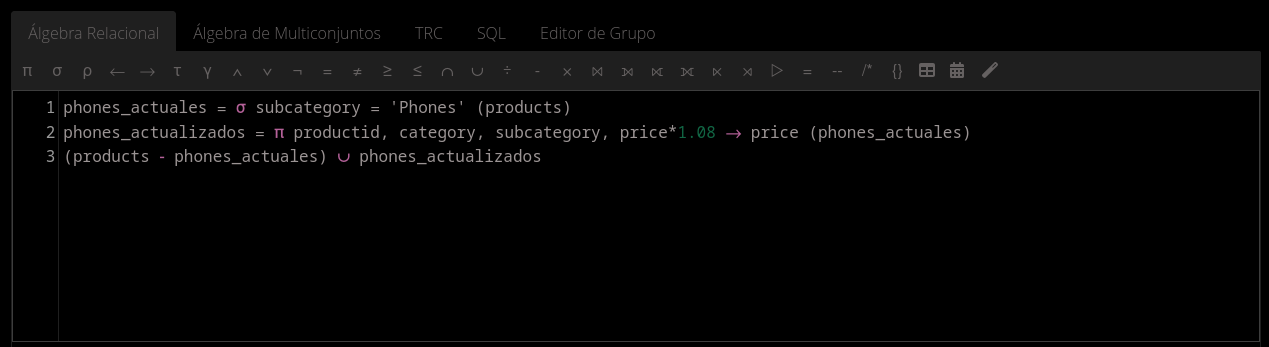
\includegraphics[width=0.8\textwidth]{imagenes/3d(1).png}
\caption{Consulta}
\end{figure}

\begin{figure}[h!]
\centering
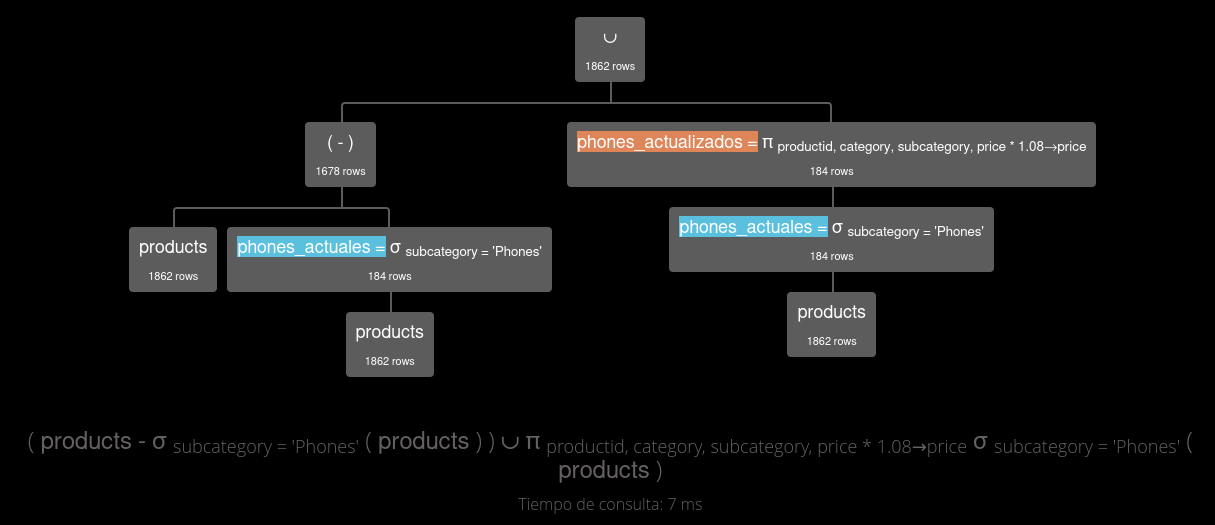
\includegraphics[width=0.8\textwidth]{imagenes/3d(2).png}
\caption{Árbol de consulta.}
\end{figure}

\begin{figure}[h!]
\centering
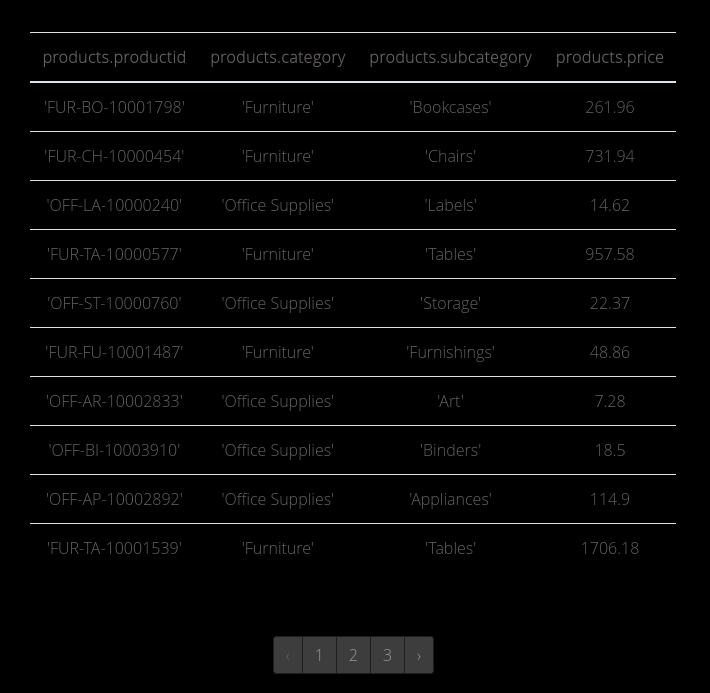
\includegraphics[width=0.6\textwidth]{imagenes/3d(3).png}
\caption{Resultado de consulta.}
\end{figure}
 \subsection*{e. Disminuir 8\% los precios de los productos de la categoría Furniture cuyo precio sea de \$600 a \$900. Aumentar en un 5\% los precios de los productos de la categoría Technology y subcategoría Machines.}

Primero filtramos los productos de la categoría \textit{Furniture} que cumplen con el rango de precios (600 a 900) mediante una selección, y guardamos el resultado como \textit{furn\_old}. Hacemos lo mismo para filtrar los productos de \textit{Technology} y subcategoría \textit{Machines}, guardándolos en \textit{tech\_old}, estos dos últimos serán los que vamos a eliminar. A continuación, utilizamos la proyección para generar las tuplas actualizadas. Para los muebles, aplicamos un descuento del 8\% multiplicando el \textit{price} por $0.92$, asignándolo al mismo nombre en \textit{furn\_new}. Para la tecnología, aplicamos el aumento del 5\% multiplicando por $1.05$ en \textit{tech\_new}. Finalmente, llevamos a cabo el mantenimiento en la relación general \textit{products}: borramos (restamos) las tuplas originales que apartamos, y unimos (insertamos) los subconjuntos nuevos calculados.

Expresión:
\begin{equation}
\begin{split}
\text{furn\_old} &= \sigma_{category = \text{'Furniture'} \, \wedge \, price \ge 600 \, \wedge \, price \le 900}(products) \\
\text{tech\_old} &= \sigma_{category = \text{'Technology'} \, \wedge \, subcategory = \text{'Machines'}}(products) \\
\text{furn\_new} &= \pi_{productid,\, category,\, subcategory,\, price \cdot 0.92 \rightarrow price}(\text{furn\_old}) \\
\text{tech\_new} &= \pi_{productid,\, category,\, subcategory,\, price \cdot 1.05 \rightarrow price}(\text{tech\_old}) \\
\text{Resultado} &= (products - \text{furn\_old} - \text{tech\_old}) \cup \text{furn\_new} \cup \text{tech\_new}
\end{split}
\end{equation}

Resultados obtenidos:

\begin{figure}[h!]
\centering
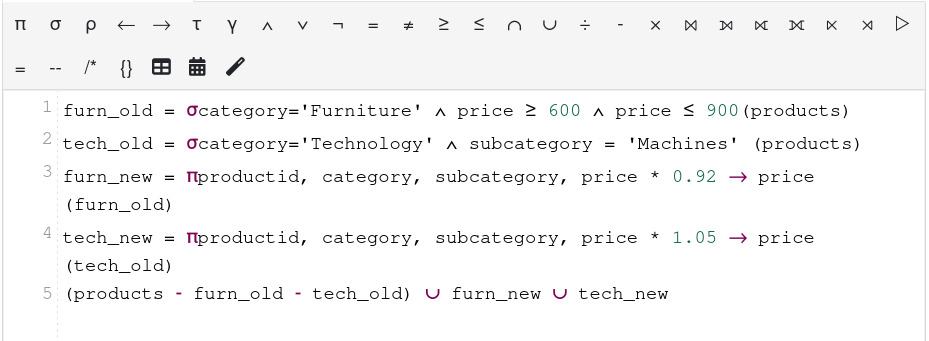
\includegraphics[width=0.8\textwidth]{imagenes/3e(1).png}
\caption{Consulta 3e.}
\end{figure}

\begin{figure}[h!]
\centering
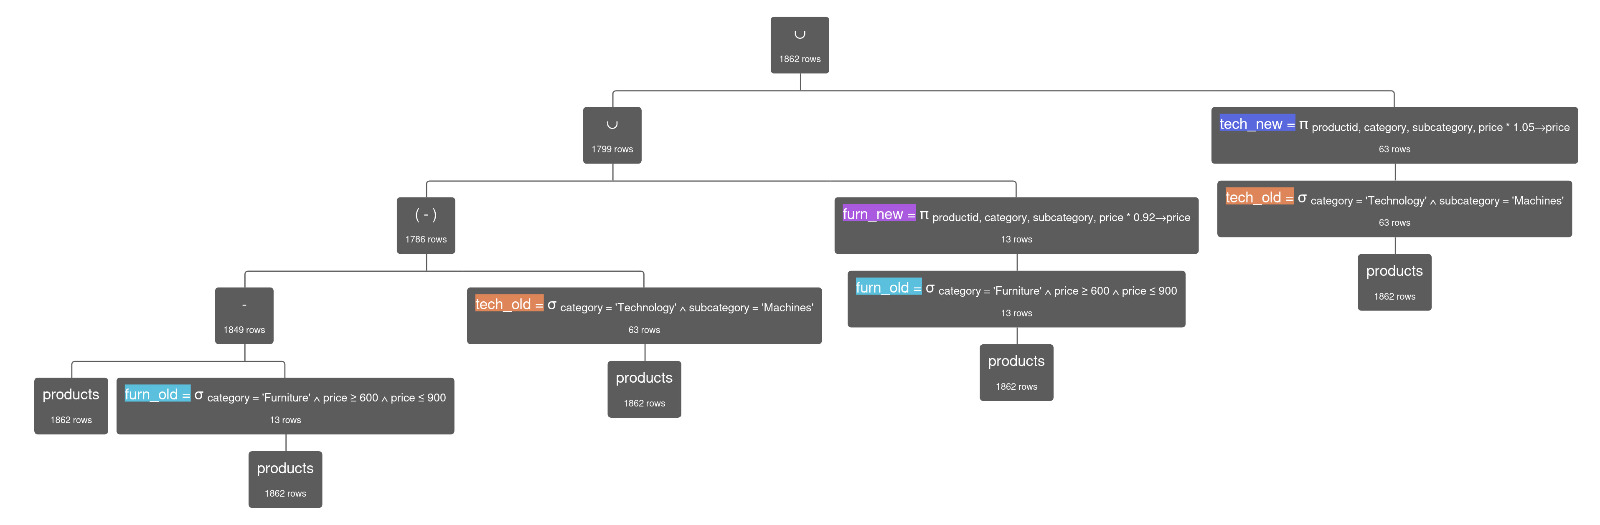
\includegraphics[width=0.8\textwidth]{imagenes/3e(2).png}
\caption{Árbol de consulta 3e.}
\end{figure}

\begin{figure}[h!]
\centering
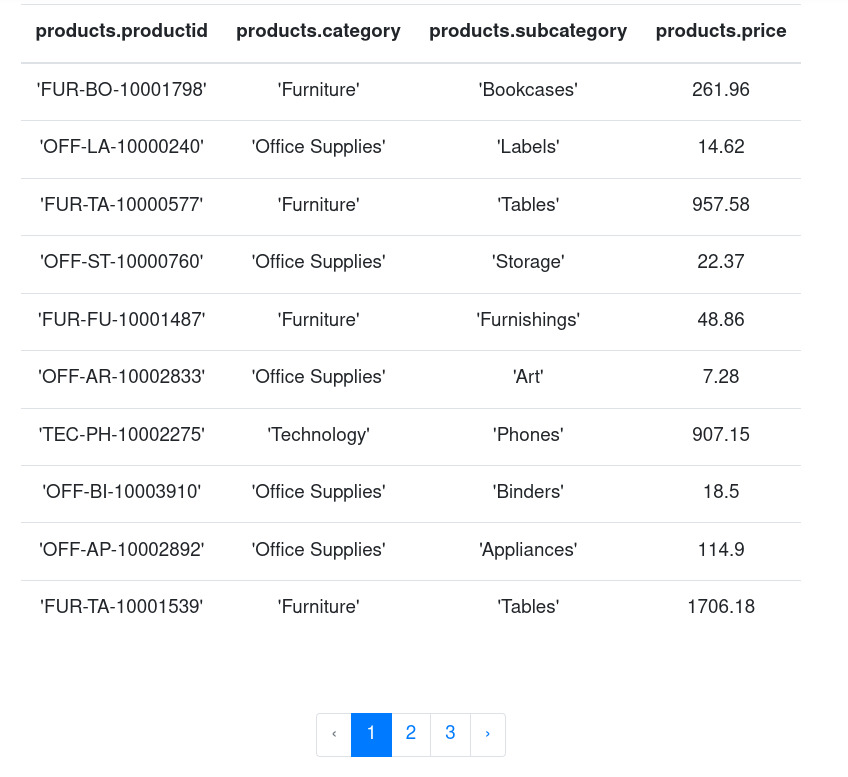
\includegraphics[width=0.6\textwidth]{imagenes/3e(3).png}
\caption{Resultado de consulta 3e.}
\end{figure}

 
 \newpage
%\nocite{*} 
%\printbibliography[title={Referencias}]

\end{document}
